% Options for packages loaded elsewhere
\PassOptionsToPackage{unicode}{hyperref}
\PassOptionsToPackage{hyphens}{url}
\PassOptionsToPackage{dvipsnames,svgnames,x11names}{xcolor}
%
\documentclass[
  letterpaper,
  DIV=11,
  numbers=noendperiod]{scrartcl}

\usepackage{amsmath,amssymb}
\usepackage{iftex}
\ifPDFTeX
  \usepackage[T1]{fontenc}
  \usepackage[utf8]{inputenc}
  \usepackage{textcomp} % provide euro and other symbols
\else % if luatex or xetex
  \usepackage{unicode-math}
  \defaultfontfeatures{Scale=MatchLowercase}
  \defaultfontfeatures[\rmfamily]{Ligatures=TeX,Scale=1}
\fi
\usepackage{lmodern}
\ifPDFTeX\else  
    % xetex/luatex font selection
    \setmainfont[]{Times New Roman}
\fi
% Use upquote if available, for straight quotes in verbatim environments
\IfFileExists{upquote.sty}{\usepackage{upquote}}{}
\IfFileExists{microtype.sty}{% use microtype if available
  \usepackage[]{microtype}
  \UseMicrotypeSet[protrusion]{basicmath} % disable protrusion for tt fonts
}{}
\makeatletter
\@ifundefined{KOMAClassName}{% if non-KOMA class
  \IfFileExists{parskip.sty}{%
    \usepackage{parskip}
  }{% else
    \setlength{\parindent}{0pt}
    \setlength{\parskip}{6pt plus 2pt minus 1pt}}
}{% if KOMA class
  \KOMAoptions{parskip=half}}
\makeatother
\usepackage{xcolor}
\setlength{\emergencystretch}{3em} % prevent overfull lines
\setcounter{secnumdepth}{-\maxdimen} % remove section numbering
% Make \paragraph and \subparagraph free-standing
\makeatletter
\ifx\paragraph\undefined\else
  \let\oldparagraph\paragraph
  \renewcommand{\paragraph}{
    \@ifstar
      \xxxParagraphStar
      \xxxParagraphNoStar
  }
  \newcommand{\xxxParagraphStar}[1]{\oldparagraph*{#1}\mbox{}}
  \newcommand{\xxxParagraphNoStar}[1]{\oldparagraph{#1}\mbox{}}
\fi
\ifx\subparagraph\undefined\else
  \let\oldsubparagraph\subparagraph
  \renewcommand{\subparagraph}{
    \@ifstar
      \xxxSubParagraphStar
      \xxxSubParagraphNoStar
  }
  \newcommand{\xxxSubParagraphStar}[1]{\oldsubparagraph*{#1}\mbox{}}
  \newcommand{\xxxSubParagraphNoStar}[1]{\oldsubparagraph{#1}\mbox{}}
\fi
\makeatother


\providecommand{\tightlist}{%
  \setlength{\itemsep}{0pt}\setlength{\parskip}{0pt}}\usepackage{longtable,booktabs,array}
\usepackage{calc} % for calculating minipage widths
% Correct order of tables after \paragraph or \subparagraph
\usepackage{etoolbox}
\makeatletter
\patchcmd\longtable{\par}{\if@noskipsec\mbox{}\fi\par}{}{}
\makeatother
% Allow footnotes in longtable head/foot
\IfFileExists{footnotehyper.sty}{\usepackage{footnotehyper}}{\usepackage{footnote}}
\makesavenoteenv{longtable}
\usepackage{graphicx}
\makeatletter
\newsavebox\pandoc@box
\newcommand*\pandocbounded[1]{% scales image to fit in text height/width
  \sbox\pandoc@box{#1}%
  \Gscale@div\@tempa{\textheight}{\dimexpr\ht\pandoc@box+\dp\pandoc@box\relax}%
  \Gscale@div\@tempb{\linewidth}{\wd\pandoc@box}%
  \ifdim\@tempb\p@<\@tempa\p@\let\@tempa\@tempb\fi% select the smaller of both
  \ifdim\@tempa\p@<\p@\scalebox{\@tempa}{\usebox\pandoc@box}%
  \else\usebox{\pandoc@box}%
  \fi%
}
% Set default figure placement to htbp
\def\fps@figure{htbp}
\makeatother
% definitions for citeproc citations
\NewDocumentCommand\citeproctext{}{}
\NewDocumentCommand\citeproc{mm}{%
  \begingroup\def\citeproctext{#2}\cite{#1}\endgroup}
\makeatletter
 % allow citations to break across lines
 \let\@cite@ofmt\@firstofone
 % avoid brackets around text for \cite:
 \def\@biblabel#1{}
 \def\@cite#1#2{{#1\if@tempswa , #2\fi}}
\makeatother
\newlength{\cslhangindent}
\setlength{\cslhangindent}{1.5em}
\newlength{\csllabelwidth}
\setlength{\csllabelwidth}{3em}
\newenvironment{CSLReferences}[2] % #1 hanging-indent, #2 entry-spacing
 {\begin{list}{}{%
  \setlength{\itemindent}{0pt}
  \setlength{\leftmargin}{0pt}
  \setlength{\parsep}{0pt}
  % turn on hanging indent if param 1 is 1
  \ifodd #1
   \setlength{\leftmargin}{\cslhangindent}
   \setlength{\itemindent}{-1\cslhangindent}
  \fi
  % set entry spacing
  \setlength{\itemsep}{#2\baselineskip}}}
 {\end{list}}
\usepackage{calc}
\newcommand{\CSLBlock}[1]{\hfill\break\parbox[t]{\linewidth}{\strut\ignorespaces#1\strut}}
\newcommand{\CSLLeftMargin}[1]{\parbox[t]{\csllabelwidth}{\strut#1\strut}}
\newcommand{\CSLRightInline}[1]{\parbox[t]{\linewidth - \csllabelwidth}{\strut#1\strut}}
\newcommand{\CSLIndent}[1]{\hspace{\cslhangindent}#1}

\usepackage{booktabs}
\usepackage{longtable}
\usepackage{array}
\usepackage{multirow}
\usepackage{wrapfig}
\usepackage{float}
\usepackage{colortbl}
\usepackage{pdflscape}
\usepackage{tabu}
\usepackage{threeparttable}
\usepackage{threeparttablex}
\usepackage[normalem]{ulem}
\usepackage{makecell}
\usepackage{xcolor}
\KOMAoption{captions}{tableheading}
\usepackage{hyperref}
\addtokomafont{disposition}{\rmfamily}
\usepackage{siunitx}
\newcommand{\aahigh}{\mathrm{AA}_{2000}}
\newcommand{\aalow}{\mathrm{AA}_{150}}
\newcommand{\aashade}{\mathrm{AA}_{\text{shade}}}
\newcommand{\aasun}{\mathrm{AA}_{\text{sun}}}
\newcommand{\aax}{$\mathrm{AA}$}
\newcommand{\aay}{\mathrm{AA}}
\newcommand{\Aamphi}{$A_{\mathrm{amphi}}$}
\newcommand{\Ahypo}{$A_{\mathrm{hypo}}$}
\newcommand{\agcurve}{$A \textendash g_\text{sw}$}
\newcommand{\aqcurve}{$A \textendash Q$}
\newcommand{\ca}{$C_\mathrm{a}$}
\newcommand{\caequals}[1]{$C_\mathrm{a} = \qty{#1}{\micro\mol\raiseto{-1}\mol}$}
\newcommand{\cabetween}[2]{#1 < $C_\mathrm{a} < \qty{#2}{\micro\mol\raiseto{-1}\mol}$}
\newcommand{\gmaxratio}{$g_\text{max,ratio}$}
\newcommand{\gmaxshade}{$g_\text{max,shade}$}
\newcommand{\gmaxsun}{$g_\text{max,sun}$}
\newcommand{\gsw}{$g_\text{sw}$}
\newcommand{\loggsw}{$\log(g_\text{sw})$}
\newcommand{\logA}{$\log(A)$}
\newcommand{\ppfd}{$\mathrm{PPFD}$}
\newcommand{\ppfdequals}[1]{$\mathrm{PPFD} = \qty{#1}{\micro\mol\raiseto{-2}\meter\raiseto{-1}\second}$}
\newcommand{\ppfdqty}[1]{$\qty{#1}{\micro\mol\raiseto{-2}\meter\raiseto{-1}\second}$}
\newcommand{\rh}{$\mathrm{RH}$}
\newcommand{\rhequals}[1]{$\mathrm{RH} = #1\%$}
\newcommand{\tleafequals}[1]{$T_\mathrm{leaf} = \qty{#1}{\degreeCelsius}$}
\makeatletter
\@ifpackageloaded{caption}{}{\usepackage{caption}}
\AtBeginDocument{%
\ifdefined\contentsname
  \renewcommand*\contentsname{Table of contents}
\else
  \newcommand\contentsname{Table of contents}
\fi
\ifdefined\listfigurename
  \renewcommand*\listfigurename{List of Figures}
\else
  \newcommand\listfigurename{List of Figures}
\fi
\ifdefined\listtablename
  \renewcommand*\listtablename{List of Tables}
\else
  \newcommand\listtablename{List of Tables}
\fi
\ifdefined\figurename
  \renewcommand*\figurename{Figure}
\else
  \newcommand\figurename{Figure}
\fi
\ifdefined\tablename
  \renewcommand*\tablename{Table}
\else
  \newcommand\tablename{Table}
\fi
}
\@ifpackageloaded{float}{}{\usepackage{float}}
\floatstyle{ruled}
\@ifundefined{c@chapter}{\newfloat{codelisting}{h}{lop}}{\newfloat{codelisting}{h}{lop}[chapter]}
\floatname{codelisting}{Listing}
\newcommand*\listoflistings{\listof{codelisting}{List of Listings}}
\makeatother
\makeatletter
\makeatother
\makeatletter
\@ifpackageloaded{caption}{}{\usepackage{caption}}
\@ifpackageloaded{subcaption}{}{\usepackage{subcaption}}
\makeatother

\usepackage{bookmark}

\IfFileExists{xurl.sty}{\usepackage{xurl}}{} % add URL line breaks if available
\urlstyle{same} % disable monospaced font for URLs
\hypersetup{
  pdftitle={Developmental plasticity to high light intensity amplifies the advantage of amphistomous leaves},
  pdfauthor={Christopher D. Muir\^{}\{1,2*\}; Wei Shen Lim\^{}\{1\}; Dachuan Wang\^{}\{1,2\}},
  colorlinks=true,
  linkcolor={blue},
  filecolor={Maroon},
  citecolor={Blue},
  urlcolor={Blue},
  pdfcreator={LaTeX via pandoc}}


\title{Developmental plasticity to high light intensity amplifies the
advantage of amphistomous leaves}
\author{Christopher D. Muir\(^{1,2*}\) \and Wei Shen
Lim\(^{1}\) \and Dachuan Wang\(^{1,2}\)}
\date{}

\begin{document}
\maketitle


\begin{center}
$^1$School of Life Sciences, University of Hawaiʻi, Mānoa, Hawaiʻi, USA\\
$^2$Department of Botany, University of Wisconsin, Madison, Wisconsin, USA\\
\medskip
*Corresponding author: cdmuir@wisc.edu\\
\medskip
ORCID: Christopher D. Muir — \href{https://orcid.org/0000-0003-2555-3878}{0000-0003-2555-3878}\\
\end{center}

\subsection{Abstract}\label{abstract}

The presence of stomata on both leaf surfaces (amphistomy) can increase
photosynthesis in C\(_3\) plants by reducing the path length for
CO\(_2\) diffusion between substomatal cavities and chloroplasts.
Amphistomatous leaves are common among herbaceous plants growing in
sunny habitats, including many crop species. This distribution of
amphistomatous leaves in nature may result from an increased
photosynthetic benefit of amphistomy under high light intensity, either
because of acclimatory, plastic, or constitutive variation in CO\(_2\)
supply or demand. We used a recently developed method to quantify
amphistomy advantage, the photosynthetic rate of an amphistomatous leaf
relative to an otherwise identical hypostomatous leaf, in 29 diverse
populations representing 14 species of wild tomatoes (\emph{Solanum}
sect. \emph{Lycopersicon} and sect. \emph{Lycopersicoides}). Plant grown
under high light intensity benefit more in terms of CO\(_2\) assimilated
for a given stomatal conductance than plants grown under low light,
regardless of measurement light intensity or native light habitat.
Developmental plasticity in leaf thickness and/or density, an adaptive
response to optimize light interception, likely affects CO\(_2\)
diffusion within the leaf, altering amphistomy advantage as a byproduct.
Developmental plasticity may therefore play an important and previously
unnoticed role in explaining the adaptive significance of amphistomy and
the distribution of amphistomatous leaves in nature.

\subsection{Main text}\label{main-text}

Stomata are microscopic pores on the surfaces of leaves and other
photosynthetic organs formed by a pair of guard cells. They are
essential for balancing carbon gained per unit water lost and permitted
vascular plants to grow tall on land by enabling access to CO\(_2\) for
photosynthetic carbon assimilation while preventing hydraulic failure in
variable environments (\emph{1}--\emph{3}). Optimal stomatal function
depends on both dynamic changes in aperture on the scale of minutes to
hours, as well as static anatomy determined by developmental plasticity
and constitutive genetic differences (\emph{4}--\emph{6}). Understanding
how stomata respond to environmental change over daily, developmental,
and evolutionary time is important for understanding adaptation
(\emph{1}, \emph{7}--\emph{12}), predicting paleoclimate from fossil
cuticles (\emph{13}--\emph{15}), and improving crops (\emph{16}).
Stomatal function contributes to global carbon and water cycles
(\emph{17}) and therefore predicting future climate (\emph{18}).

Despite extensive theoretical and empirical progress understanding
stomata function and anatomy from molecular to ecosystem levels, the
adaptive significance of amphistomatous leaves remains an important
unsolved problem in leaf structure-function relationships
(\emph{19}--\emph{26}). Amphistomatous leaves develop abaxial and
adaxial stomata whose aperture can be independently regulated
(\emph{27}--\emph{31}) to control gas exchange through each surface. All
else being equal, gas exchange through stomata on both surfaces
increases CO\(_2\) supply to chloroplasts by providing a second parallel
pathway through leaf intercellular airspaces, enhancing photosynthesis
(\emph{20}, \emph{32}). The extent to which amphistomy increases
CO\(_2\) supply depends on resistance to diffusion in intercellular
airspaces. This resistance can be low in thin, porous, amphistomatous
leaves (\emph{28}, \emph{33}), but may be more substantial in thick,
dense, hypostomatous leaves (\emph{34}). Amphistomatous leaves also lose
more water through evaporation because of a second boundary layer
conductance (\emph{35}), but the additional carbon gain should be enough
to offset this cost in most realistic scenarios (\emph{36}).

The paradoxical fact is that, despite the photosynthetic benefit, most
leaves are not amphistomatous. Many vertically oriented and/or
isobilateral leaves are amphistomatous (\emph{25}). But among
dorsiventral leaves, herbaceous plants in open, high light habitats tend
to have have amphistomatous leaves (\emph{22}, \emph{39}--\emph{44}).
Most other leaves, except those from aquatic habitats, are
hypostomatous, producing stomata only on the lower, abaxial surface.
Even resupinate leaves develop stomata on the lower, albeit adaxial
surface (\emph{45}), suggesting that leaf orientation (lower vs.~upper)
rather than leaf polarity (abaxial vs.~adaxial) is causal. The
covariation between stomatal density ratio and light habitat is both
qualitative and quantitative. A higher proportion of sun leaves are
amphistomatous (\emph{39}) and the proportion of stomata on the upper,
adaxial surface increases with light (\emph{42}, \emph{43}). Resolving
why high light intensity favors amphistomatous dorsivental leaves is an
important first step toward understanding variation in stomatal density
ratio and leaf structure-function relationships more generally.

The overarching hypothesis is that leaves with greater stomatal density
ratio are more common in open, sunny habitats because they increase
photosynthesis most in those circumstances. An amphistomatous leaf
increases photosynthetic carbon gain compared to an otherwise identical
hypostomatous leaf by increasing conductance through the leaf
intercellular airspaces and boundary layers; the additional water loss
through a second boundary layer is typically small (\emph{35}). We
quantify this benefit as the amphistomy advantage (\aax{}), the
log-response ratio of photosynthesis in an amphistomatous leaf compared
to an otherwise identical pseudohypostomatous leaf (\emph{20},
\emph{46}). Why would \aax{} be greater in sun than shade? We consider
three nonmutually exclusive hypotheses that we classify as
`acclimatory', `plastic', and `constitutive' (Fig.~\ref{fig-concept}).

\emph{Acclimatory hypothesis}: Photosynthetic induction to high light
intensity typically involves increases in total leaf stomatal
conductance (increased CO\(_2\) supply), the concentration of active
Rubisco, and electron transport capacity (increased CO\(_2\) demand). A
one-dimensional circuit model using the Farquhar-von Caemmerer-Berry
biochemical model of C\(_3\) photosynthesis (\emph{47}) shows that both
increased stomatal conductance and Rubisco activity should increase
\aax{}, all else being equal (Supporting Information). If the
acclimatory hypothesis is correct, we predict that
\(\aahigh{} > \aalow{}\) for all populations regardless of native
habitat or growth environment.

\emph{Plasticity hypothesis}: Individuals of the same genotype often
develop dramatically different leaves in sun and shade conditions
(\emph{48}). Plastic responses are likely adaptations to optimize
photosynthesis at different light intensities in variable environments
(\emph{49}). Plastic changes in leaf anatomy and biochemistry could
modulate \aax{} as a byproduct. Thicker or less porous leaves, both of
which are associated with high leaf mass per area (LMA), will have lower
\(g_\mathrm{ias}\); leaves with increased total stomatal density and
photosynthetic capacity have greater potential CO\(_2\) supply and
demand. Under the plastic hypothesis, we predict that
\(\aasun{} > \aashade{}\) for all populations and light intensities.
Secondarily, \(\aasun{}\) and \gmaxsun{} should also be positively
associated with native light habitat if genotypes adapted to sunny, open
habitats if they can express a phenotype best adapted to that
environment when leaves develop under high light intensity.

\emph{Constitutive hypothesis}: In environments that are relatively
constant or where environmental change cannot be anticipated by a
reliable cue, natural selection will favor constitutive expression of
optimal phenotypes. We therefore predict genotypes from more sunny, open
habitats will have consistently greater \aax under also measurement and
growth light intensities. For herbaceous plants, light intensity is
largely a function of the tree canopy (\emph{50}). Herbs growing in the
open will regularly experience high light intensity; herbs growing under
a forest canopy will often experience low light intensity.

\begin{figure}

\centering{

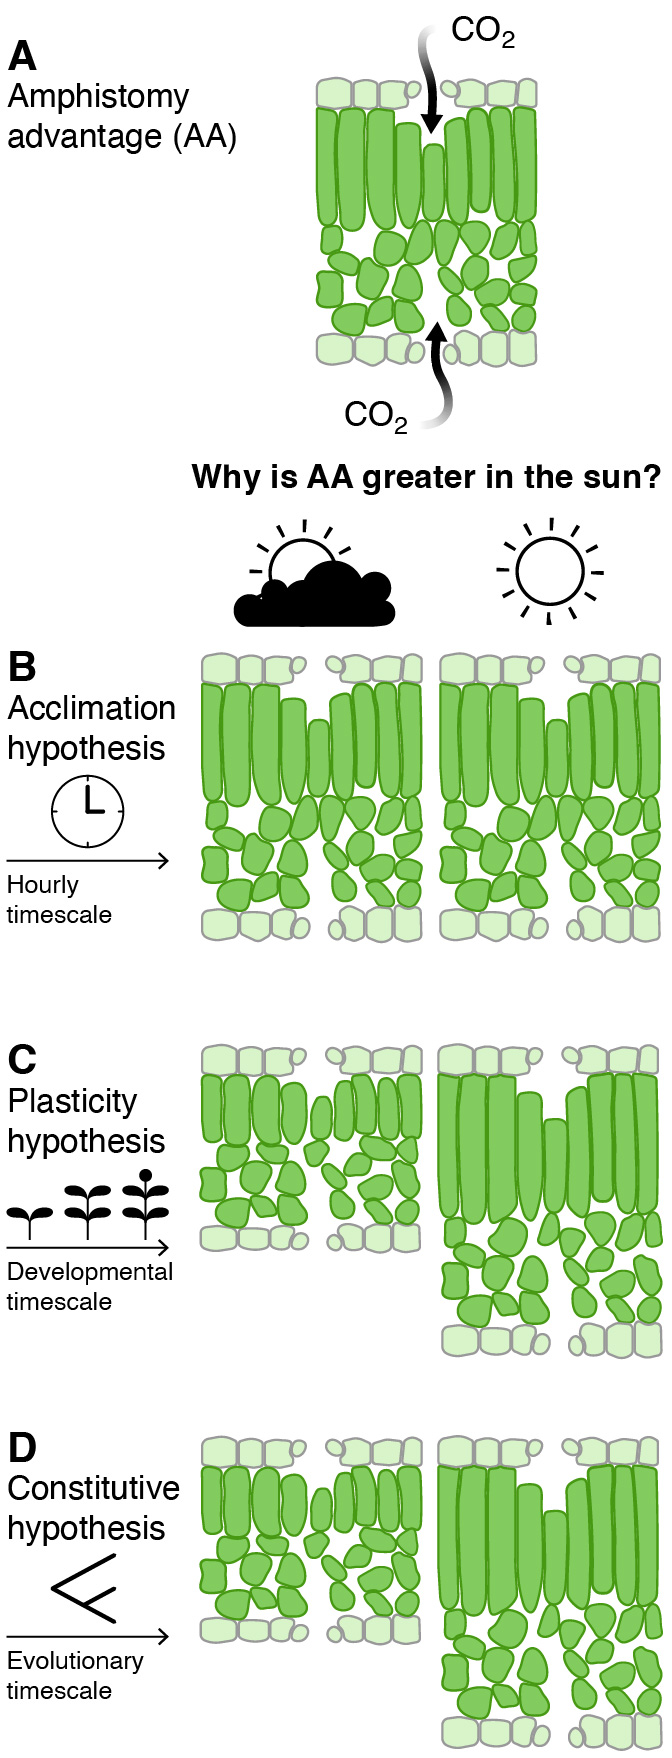
\includegraphics[width=2.24in,height=\textheight,keepaspectratio]{../figures/amphisomy draft 2024-03-28.jpg}

}

\caption{\label{fig-concept}\textbf{Conceptual outline of three nonmutually exclusive hypotheses explaining why amphistomy advantage (\aax{}) might be greater for leaves in sunny, open habitats.}
The acclimatory hypothesis predicts that \aax{} is greater under high
measurement light intensity (\ppfdqty{2000}) than low measurement light
intensity (\ppfdequals{150}), regardless of growth light intensity or
native plant area index (PAI). The plasticity hypothesis predicts that
\aax{} is greater for plants grown in sun than shade, regardless of
measurement light intensity or native PAI. The constitutive hypothesis
predicts that \aax{} is greater for plants adapted to sunny habitats
(lower native PAI) than shaded habitats, regardless of measurement light
intensity or growth light intensity.}

\end{figure}%

The primary directional predictions for each hypothesis are summarized
in Table~\ref{tbl-hypotheses}; detailed predictions for results that
would indicate support for multiple hypotheses are in
Table~\ref{tbl-predictions}.

\begin{table}

\caption{\label{tbl-hypotheses}Three nonmutually exclusive hypotheses
and directional predictions explaining why amphistomy advantage (\aax{})
might be greater for leaves in sunny, open habitats. For each
hypothesis, we make predictions for how measurement light intensity
(\ppfdequals{150} vs.~\ppfdqty{2000}), growth light intensity (sun
vs.~shade), and native plant area index (PAI) would affect \aax{}.
\ppfd{}: photosynthetic photon flux density.}

\centering{

\centering
\begin{tabular}{>{\centering\arraybackslash}p{1in}>{\centering\arraybackslash}p{1.5in}>{\centering\arraybackslash}p{1.5in}>{\centering\arraybackslash}p{1.25in}}
\toprule
Hypothesis & Measurement light intensity & Growth light intensity & Native PAI\\
\midrule
acclimatory & $\mathrm{AA}_{2000} > \mathrm{AA}_{150}$ & $\mathrm{AA}_{\text{sun}} = \mathrm{AA}_{\text{shade}}$ & $\operatorname{cor}(\mathrm{PAI}, \mathrm{AA}) = 0$\\
plastic & $\mathrm{AA}_{2000} = \mathrm{AA}_{150}$ & $\mathrm{AA}_{\text{sun}} > \mathrm{AA}_{\text{shade}}$ & $\operatorname{cor}(\mathrm{PAI}, \mathrm{AA}) = 0$\\
constitutive & $\mathrm{AA}_{2000} = \mathrm{AA}_{150}$ & $\mathrm{AA}_{\text{sun}} = \mathrm{AA}_{\text{shade}}$ & $\operatorname{cor}(\mathrm{PAI}, \mathrm{AA}) > 0$\\
\bottomrule
\end{tabular}

}

\end{table}%

We tested these hypotheses by comparing \aax{} among amphistomatous wild
tomato species (\emph{51}) from different native light habitats, grown
under simulated sun and shade light treatments, and measured under
contrasting light intensities (low and high). We measured \aax{} on 572
individual plants from 29 populations (average of 9.86 replicates per
light treatment) using a recently developed method (\emph{46}). With
this method, we directly compare the photosynthetic rate of an untreated
amphistomatous leaf to that of the same leaf with gas exchange blocked
through the adaxial (upper) surface by transparent plastic, which we
refer to as `pseudohypostomy'. To compare amphi- and pseudohypostomatous
leaves at identical whole-leaf \(g_\text{sc}\), we measure \(A\) over a
range of \(g_\text{sc}\), inducing stomatal opening and closure by
modulating humidity (see Materials and Methods for further details). We
estimated `amphistomy advantage' (\aax) \emph{sensu} (\emph{20}), but
with modifications previously described in (\emph{46}) and here
(Materials and Methods). The native light intensity was represented by
plant area index (PAI \(\unit{\meter\squared\per\meter\squared}\)),
estimated using a global gridded data set derived from the Global
Ecosystem Dynamics Investigation {[}GEDI; (\emph{52}){]} and
georeferenced accession collection information from the Tomato Genetics
Resource Center. The growth light intensities were \ppfdequals{761} (sun
treatment) and \ppfdqty{115} (shade treatment) while all other
environment conditions were nearly identical (see Materials and
Methods). The high and low measurement light intensities were
\ppfdequals{2000} (97.8:2.24 red:blue) and \ppfdequals{150} (87.0:13.0
red:blue), respectively.

Consistent with biophysical theory of CO\(_2\) diffusion within leaves,
\(\aay{} > 0\) for all populations (Fig.~\ref{fig-aa}A). Bayesian
phylogenetic mixed effects models that allowed \aax{} to vary between
measurement light intensities, growth light intensities, and among
populations outperformed simpler models based on information criteria
(Table~\ref{tbl-aa_loo1}). Measured under high light intensity, \aax{}
was consistently greater for sun plants. The average \aax{} among
populations in the shade treatment was 0.041 (range: 0.007--0.113; 19 of
29 populations significant); however, the same populations grown at high
light intensity showed a mean \aax{} of 0.052 (range: 0.020--0.120; 20
of 29 populations significant). Contrary to the predictions of the
assimilatory hypothesis, \aax{} was greater in all populations under low
measurement light intensity for both sun and shade grown plants. The
effect of low light on \aax{} was more pronounced in the sun-grown
plants, where \aax{} was significantly greater under low measurement
light intensity in 13 of 29 populations compared to 12 populations for
shade-grown plants. The overall average \aax{} of shade and sun grown
plants measured under low light intensity was 0.064 (range:
0.022--0.137; 28 of 29 populations significant) and 0.100 (range:
0.049--0.206; 27 of 29 populations significant), respectively. There was
a modest tendency for populations from more open habitats (lower PAI) to
exhibit greater \aax{} and the slope was significantly different than 0
in 3 of the 4 treatment combinations (Fig.~\ref{fig-aa}B).

\begin{figure}

\centering{

\pandocbounded{\includegraphics[keepaspectratio]{ms_files/figure-pdf/fig-aa-1.pdf}}

}

\caption{\label{fig-aa}Caption on following page.}

\end{figure}%

\addtocounter{figure}{-1}

\begin{figure}

\centering{

\pandocbounded{\includegraphics[keepaspectratio]{ms_files/figure-pdf/fig-aacap-1.pdf}}

}

\caption{\label{fig-aacap}\textbf{Amphistomy advantage (\aax{}) in greater wild tomatoes from open habitats and is further amplified by developmental plasticity under sunny growth conditions.}
\aax{} (\(y\)-axis) is the log-response ratio of photosynthesis in an
amphistomatous leaf compared to an otherwise identical
pseudohypostomatous leaf. In both panels, estimates are shown for plants
grown under simulated shade (brown) or sun (orange) and measured under
high light intensity (\ppfdequals{2000}; open circles) and low light
intensity (\ppfdequals{150}; solid circles). The dashed line at zero
indicates no difference in photosynthesis between amphi- and
pseudohypostomatous leaves. (\textbf{A}) The points are the posterior
median \aax{} for each population, with error bars showing 95\%
confidence intervals. Within each facet, the populations are arranged by
\aax{} estimated in that growth and measurement condition. The average
\aax{} among populations for each treatment group is written in the top
left corner. (\textbf{B}) The same estimates of \aax{} in each
combination of growth and measurement light intensity ploted against
native plant area index (PAI; \(x\)-axis, log-scale). The confidence
intervals were omitted for visual clarity. The median relationship
between native PAI (\(x\)-axis; log-scale) and \aax{} is shown as a
solid line with the shaded region between dashed lines showing the 95\%
confidence ribbon. The * in the top left corner of each facet indicates
the slope of the linear regression is significantly different from zero;
n.s. indicates not significant.}

\end{figure}%

\subsubsection{MARKER - where is evidence for relationship between PAI
and LMA,
AA?}\label{marker---where-is-evidence-for-relationship-between-pai-and-lma-aa}

The pattern of \aax{} across wild tomatoes strongly supports the
plasticity hypothesis, argues against the acclimatory hypothesis, and
provides modest support for the constitutive hypothesis. Plastic changes
in leaf thickness and/or packing density, summarized by the bulk leaf
mass per area (LMA), may mediate the effect of growth light intensity on
\aax{}. LMA increased in sun grown plants in all populations by an
average of 123\% {[}95\% CI: 42.9 to 256\%{]}, similar to plastic
responses in many species (\emph{48}). While LMA is weakly, albeit
significantly, associated with individual-level \aax{}
(Fig.~\ref{fig-lma_aa}), the effect of growth light intensity on \aax{}
is still predictive based on model comparison (Table~\ref{tbl-aa_loo1}).
In contrast, LMA did not mediate an indirect effect of native PAI on
\aax{} (Table/Figure). Many anatomical traits underlie LMA (\emph{53})
and future research will be needed identify which particular traits,
such as leaf thickness or mesophyll porosity, are responsible for
mediating \aax{}. The fact that the \aax{} of sun plants was greater
under low measurement light intensity supports a long-standing
hypothesis that resistance to CO\(_2\) diffusion is greater in the upper
than lower portions of the leaf interior (\emph{54}). At low light
intensity, the bulk properties of the leaf are weighed toward the upper
palisade where most light is intercepted. Hence, amphistomy may,
unexpectedly, be particularly beneficial for sun leaves experiencing
intermittent shade or cloud cover. Our study is limited in testing this
because we could not directly measure the stomatal conductance ratio and
intercellular resistance on each surface. Future experiments measuring
\aax{} with a dual sided chamber (\emph{31}, \emph{33}) can overcome
these limitations.

\begin{figure}

\centering{

\pandocbounded{\includegraphics[keepaspectratio]{ms_files/figure-pdf/fig-lma_aa-1.pdf}}

}

\caption{\label{fig-lma_aa}\textbf{Plastic changes in leaf mass per area (LMA) mediate the effect of sun- to shade-grown plants on amphistomy advantage (\aax{}).}
Each point is the estimated population-level LMA (\(x\)-axis) and \aax{}
(\(y\)-axis) for each population grown under high light intensity
(\ppfdequals{2000}) and low light intensity (\ppfdequals{150}). The
points are colored by growth light treatment. The solid line is the
posterior median of the linear regression of individual-level LMA on
\(\aahigh\) with the shaded region showing the 95\% confidence ribbon;
the dashed line is the same for \(\aalow\). Confidence intervals for
each population estimate and individual-level estimates are omitted for
visual clarity.}

\end{figure}%

We conclude that developmental plasticity, as opposed to acclimation or
adaptation to open habitats, may explain the explain the long-standing
observation that amphistomatous leaves are more common in sunny
habitats, at least among herbaceous plants including crop relatives. Our
results advance existing explanations by showing high light intensity
\emph{per se} does not increase the benefit of amphistomy, but rather
that anatomical and biochemical change associated with higher light
intensity modulate \aax{}. Developmental plasticity needs to be
considered when interpreting phylogenetic comparative analyses of
adaptation, because plastic differences may be mistaken for genetic
differences.

maybe this wording is better: Amphistomy likely plays a significant, but
under appreciated, role in the carbon and water balance of plant groups
where this trait is common, such as herbaceous plants in sunny habitats
and woody species in arid biomes (cites). If our estimates of AA from
the wild tomato clades

note: estimates of AA are less than that described by Parkhurst and Mott
(1990) and also less than that of Xiong and Flexas (2021). What does
this tell us?

A second major conclusion is that the significant photosynthetic gain of
amphistomatous leaves implies that the many hypostomatous leaves that
dominate mesic to wet forests globally are giving up `free' carbon that
would require little to no additional water loss. Under realistic
assumptions, we estimate that hypostomatous leaves could achieve the
same \(A\) with X to X\% less water loss if they were amphistomatous
(Table S9). Ours is the first experimental demonstration that amphistomy
is beneficial for sun leaves because of plastic changes, but future
research needs to estimates the tradeoffs associated with amphistomatous
leaves in order to fully explain their rarity among many woody plants
and shade-tolerant herbs.

\subsection{Acknowledgements}\label{acknowledgements}

Sam McKlin and Tom Buckley helped with protocol development. Justin
Alter, Max Gatlin, Joana Kim, Jenna Matsuyama, Brandon Najarian, and Kai
Yasuda contributed to data collection. Sarah Friedrich helped with
conceptual figure.

\subsubsection{Funding:}\label{funding}

US National Science Foundation OIA-1929167 to C.D.M.

\subsubsection{Author contributions:}\label{author-contributions}

Conceptualization: C.D.M.; Methodology: C.D.M., W.S.L.; Investigation:
C.D.M., W.S.L., D.W.; Visualization: C.D.M.; Funding acquisition:
C.D.M.; Writing -- original draft: C.D.M.; Writing -- review \& editing:
C.D.M., W.S.L., D.W.

\subsection{References}\label{references}

\phantomsection\label{refs}
\begin{CSLReferences}{0}{1}
\bibitem[\citeproctext]{ref-raven_selection_2002}
\CSLLeftMargin{1. }%
\CSLRightInline{J. A. Raven,
\href{https://doi.org/10.1046/j.0028-646X.2001.00334.x}{Selection
pressures on stomatal evolution}. \emph{New Phytologist} \textbf{153},
371--386 (2002).}

\bibitem[\citeproctext]{ref-mcadam_stomata_2021}
\CSLLeftMargin{2. }%
\CSLRightInline{S. A. M. McAdam, J. G. Duckett, F. C. Sussmilch, S.
Pressel, K. S. Renzaglia, R. Hedrich, T. J. Brodribb, A. Merced,
\href{https://doi.org/10.1002/ajb2.1619}{Stomata: The holey grail of
plant evolution}. \emph{American Journal of Botany} \textbf{108},
366--371 (2021).}

\bibitem[\citeproctext]{ref-clark_origin_2022}
\CSLLeftMargin{3. }%
\CSLRightInline{J. W. Clark, B. J. Harris, A. J. Hetherington, N.
Hurtado-Castano, R. A. Brench, S. Casson, T. A. Williams, J. E. Gray, A.
M. Hetherington, \href{https://doi.org/10.1016/j.cub.2022.04.040}{The
origin and evolution of stomata}. \emph{Current Biology} \textbf{32},
R539--R553 (2022).}

\bibitem[\citeproctext]{ref-hetherington_role_2003}
\CSLLeftMargin{4. }%
\CSLRightInline{A. M. Hetherington, F. I. Woodward,
\href{https://doi.org/10.1038/nature01843}{The role of stomata in
sensing and driving environmental change}. \emph{Nature} \textbf{424},
901--908 (2003).}

\bibitem[\citeproctext]{ref-de_boer_optimal_2016}
\CSLLeftMargin{5. }%
\CSLRightInline{H. J. de Boer, C. A. Price, F. Wagner‐Cremer, S. C.
Dekker, P. J. Franks, E. J. Veneklaas,
\href{https://doi.org/10.1111/nph.13929}{Optimal allocation of leaf
epidermal area for gas exchange}. \emph{New Phytologist} \textbf{210},
1219--1228 (2016).}

\bibitem[\citeproctext]{ref-harrison_influence_2020}
\CSLLeftMargin{6. }%
\CSLRightInline{E. L. Harrison, L. Arce Cubas, J. E. Gray, C. Hepworth,
\href{https://doi.org/10.1111/tpj.14560}{The influence of stomatal
morphology and distribution on photosynthetic gas exchange}. \emph{The
Plant Journal} \textbf{101}, 768--779 (2020).}

\bibitem[\citeproctext]{ref-woodward_stomatal_1987}
\CSLLeftMargin{7. }%
\CSLRightInline{F. I. Woodward,
\href{https://doi.org/10.1038/327617a0}{Stomatal numbers are sensitive
to increases in {CO2} from pre-industrial levels}. \emph{Nature}
\textbf{327}, 617--618 (1987).}

\bibitem[\citeproctext]{ref-buckley_modelling_2013}
\CSLLeftMargin{8. }%
\CSLRightInline{T. N. Buckley, K. A. Mott,
\href{https://doi.org/10.1111/pce.12140}{Modelling stomatal conductance
in response to environmental factors: {Modelling} stomatal conductance}.
\emph{Plant, Cell \& Environment} \textbf{36}, 1691--1699 (2013).}

\bibitem[\citeproctext]{ref-haworth_co-ordination_2013}
\CSLLeftMargin{9. }%
\CSLRightInline{M. Haworth, C. Elliott-Kingston, J. C. McElwain,
\href{https://doi.org/10.1007/s00442-012-2406-9}{Co-ordination of
physiological and morphological responses of stomata to elevated
{[}{CO2}{]} in vascular plants}. \emph{Oecologia} \textbf{171}, 71--82
(2013).}

\bibitem[\citeproctext]{ref-liang_stomatal_2023}
\CSLLeftMargin{10. }%
\CSLRightInline{X. Liang, D. Wang, Q. Ye, J. Zhang, M. Liu, H. Liu, K.
Yu, Y. Wang, E. Hou, B. Zhong, L. Xu, T. Lv, S. Peng, H. Lu, P. Sicard,
A. Anav, D. S. Ellsworth,
\href{https://doi.org/10.1038/s41467-023-37934-7}{Stomatal responses of
terrestrial plants to global change}. \emph{Nature Communications}
\textbf{14}, 2188 (2023).}

\bibitem[\citeproctext]{ref-chua_stomatal_2024}
\CSLLeftMargin{11. }%
\CSLRightInline{L. C. Chua, O. S. Lau,
\href{https://doi.org/10.1242/dev.202681}{Stomatal development in the
changing climate}. \emph{Development} \textbf{151}, dev202681 (2024).}

\bibitem[\citeproctext]{ref-lang_century-long_2024}
\CSLLeftMargin{12. }%
\CSLRightInline{P. L. M. Lang, J. M. Erberich, L. Lopez, C. L. Weiß, G.
Amador, H. F. Fung, S. M. Latorre, J. R. Lasky, H. A. Burbano, M.
Expósito-Alonso, D. C. Bergmann,
\href{https://doi.org/10.1038/s41559-024-02481-x}{Century-long timelines
of herbarium genomes predict plant stomatal response to climate change}.
\emph{Nature Ecology \& Evolution} \textbf{8}, 1641--1653 (2024).}

\bibitem[\citeproctext]{ref-franks_new_2014}
\CSLLeftMargin{13. }%
\CSLRightInline{P. J. Franks, D. L. Royer, D. J. Beerling, P. K. Van de
Water, D. J. Cantrill, M. M. Barbour, J. A. Berry,
\href{https://doi.org/10.1002/2014GL060457}{New constraints on
atmospheric {CO}\(_{\textrm{2}}\) concentration for the {Phanerozoic}}.
\emph{Geophysical Research Letters} \textbf{41}, 4685--4694 (2014).}

\bibitem[\citeproctext]{ref-mcelwain_paleoecology_2017}
\CSLLeftMargin{14. }%
\CSLRightInline{J. C. McElwain, M. Steinthorsdottir, Paleoecology,
ploidy, paleoatmospheric composition, and developmental biology: A
review of the multiple uses of fossil stomata. \emph{Plant Physiology}
\textbf{174}, 650--664 (2017).}

\bibitem[\citeproctext]{ref-the_cenozoic_co_proxy_integration_project_cencopip_consortium_toward_2023}
\CSLLeftMargin{15. }%
\CSLRightInline{The Cenozoic CO Proxy Integration Project (CenCOPIP)
Consortium*†, B. Hönisch, D. L. Royer, D. O. Breecker, P. J. Polissar,
G. J. Bowen, M. J. Henehan, Y. Cui, M. Steinthorsdottir, J. C. McElwain,
M. J. Kohn, A. Pearson, S. R. Phelps, K. T. Uno, A. Ridgwell, E.
Anagnostou, J. Austermann, M. P. S. Badger, R. S. Barclay, P. K. Bijl,
T. B. Chalk, C. R. Scotese, E. De La Vega, R. M. DeConto, K. A. Dyez, V.
Ferrini, P. J. Franks, C. F. Giulivi, M. Gutjahr, D. T. Harper, L. L.
Haynes, M. Huber, K. E. Snell, B. A. Keisling, W. Konrad, T. K.
Lowenstein, A. Malinverno, M. Guillermic, L. M. Mejía, J. N. Milligan,
J. J. Morton, L. Nordt, R. Whiteford, A. Roth-Nebelsick, J. K. C.
Rugenstein, M. F. Schaller, N. D. Sheldon, S. Sosdian, E. B. Wilkes, C.
R. Witkowski, Y. G. Zhang, L. Anderson, D. J. Beerling, C. Bolton, T. E.
Cerling, J. M. Cotton, J. Da, D. D. Ekart, G. L. Foster, D. R.
Greenwood, E. G. Hyland, E. A. Jagniecki, J. P. Jasper, J. B. Kowalczyk,
L. Kunzmann, W. M. Kürschner, C. E. Lawrence, C. H. Lear, M. A.
Martínez-Botí, D. P. Maxbauer, P. Montagna, B. D. A. Naafs, J. W. B.
Rae, M. Raitzsch, G. J. Retallack, S. J. Ring, O. Seki, J. Sepúlveda, A.
Sinha, T. F. Tesfamichael, A. Tripati, J. Van Der Burgh, J. Yu, J. C.
Zachos, L. Zhang, \href{https://doi.org/10.1126/science.adi5177}{Toward
a {Cenozoic} history of atmospheric {CO}\(_{\textrm{2}}\)}.
\emph{Science} \textbf{382}, eadi5177 (2023).}

\bibitem[\citeproctext]{ref-hofmann_impact_2025}
\CSLLeftMargin{16. }%
\CSLRightInline{T. A. Hofmann, W. Atkinson, M. Fan, A. J. Simkin, P.
Jindal, T. Lawson, \href{https://doi.org/10.1098/rstb.2024.0244}{Impact
of climate-driven changes in temperature on stomatal anatomy and
physiology}. \emph{Philosophical Transactions of the Royal Society B:
Biological Sciences} \textbf{380}, 20240244 (2025).}

\bibitem[\citeproctext]{ref-berry_stomata:_2010}
\CSLLeftMargin{17. }%
\CSLRightInline{J. A. Berry, D. J. Beerling, P. J. Franks,
\href{https://doi.org/10.1016/j.pbi.2010.04.013}{Stomata: Key players in
the earth system, past and present}. \emph{Current Opinion in Plant
Biology} \textbf{13}, 232--239 (2010).}

\bibitem[\citeproctext]{ref-franks_stomatal_2017}
\CSLLeftMargin{18. }%
\CSLRightInline{P. J. Franks, J. A. Berry, D. L. Lombardozzi, G. B.
Bonan, \href{https://doi.org/10.1104/pp.17.00287}{Stomatal {Function}
across {Temporal} and {Spatial} {Scales}: {Deep}-{Time} {Trends},
{Land}-{Atmosphere} {Coupling} and {Global} {Models}}. \emph{Plant
Physiology} \textbf{174}, 583--602 (2017).}

\bibitem[\citeproctext]{ref-grubb_leaf_1977}
\CSLLeftMargin{19. }%
\CSLRightInline{P. J. Grubb, {``Leaf structure and function''} in
\emph{The Encyclopedia of Ignorance}, R. Duncan, M. Weston-Smith, Eds.
(Pergamon, Oxford, 1977)vol. 2, pp. 317--330.}

\bibitem[\citeproctext]{ref-parkhurst_adaptive_1978}
\CSLLeftMargin{20. }%
\CSLRightInline{D. F. Parkhurst,
\href{https://doi.org/10.2307/2259142}{The adaptive significance of
stomatal occurrence on one or both surfaces of leaves}. \emph{The
Journal of Ecology} \textbf{66}, 367--383 (1978).}

\bibitem[\citeproctext]{ref-mott_adaptive_1982}
\CSLLeftMargin{21. }%
\CSLRightInline{K. A. Mott, A. C. Gibson, J. W. O'Leary,
\href{https://doi.org/10.1111/1365-3040.ep11611750}{The adaptive
significance of amphistomatic leaves}. \emph{Plant, Cell \& Environment}
\textbf{5}, 455--460 (1982).}

\bibitem[\citeproctext]{ref-gibson_structure-function_1996}
\CSLLeftMargin{22. }%
\CSLRightInline{A. C. Gibson, \emph{Structure-{Function} {Relations} of
{Warm} {Desert} {Plants}} (Springer Berlin / Heidelberg, Berlin,
Heidelberg, 1996;
\url{http://public.eblib.com/choice/PublicFullRecord.aspx?p=6495247}).}

\bibitem[\citeproctext]{ref-smith_leaf_1997}
\CSLLeftMargin{23. }%
\CSLRightInline{W. K. Smith, T. C. Vogelmann, E. H. DeLucia, D. T. Bell,
K. A. Shepherd, \href{https://doi.org/10.2307/1313100}{Leaf {Form} and
{Photosynthesis}}. \emph{BioScience} \textbf{47}, 785--793 (1997).}

\bibitem[\citeproctext]{ref-oguchi_leaf_2018}
\CSLLeftMargin{24. }%
\CSLRightInline{R. Oguchi, Y. Onoda, I. Terashima, D. Tholen, {``Leaf
{Anatomy} and {Function}''} in \emph{The {Leaf}: {A} {Platform} for
{Performing} {Photosynthesis}}, W. W. Adams III, I. Terashima, Eds.
(Springer International Publishing, Cham, 2018;
\url{https://doi.org/10.1007/978-3-319-93594-2_5})\emph{Advances in
{Photosynthesis} and {Respiration}}, pp. 97--139.}

\bibitem[\citeproctext]{ref-drake_two_2019}
\CSLLeftMargin{25. }%
\CSLRightInline{P. L. Drake, H. J. de Boer, S. J. Schymanski, E. J.
Veneklaas, \href{https://doi.org/10.1111/nph.15652}{Two sides to every
leaf: Water and {CO}\(_{\textrm{2}}\) transport in hypostomatous and
amphistomatous leaves}. \emph{New Phytologist} \textbf{222}, 1179--1187
(2019).}

\bibitem[\citeproctext]{ref-grubb_leaf_2020}
\CSLLeftMargin{26. }%
\CSLRightInline{P. J. Grubb, {``Leaf structure and function''} in
\emph{Unsolved {Problems} in {Ecology}}, A. Dobson, D. Tilman, R. D.
Holt, Eds. (Princeton University Press, Princeton, 2020), pp. 124--144.}

\bibitem[\citeproctext]{ref-pospisilova_environmental_1980}
\CSLLeftMargin{27. }%
\CSLRightInline{J. Pospíŝilová, J. Solárová, Environmental and
biological control of diffusive conductances of adaxial and abaxial leaf
epidermes. \emph{Photosynthetica} \textbf{14}, 90--127 (1980).}

\bibitem[\citeproctext]{ref-mott_stomatal_1984}
\CSLLeftMargin{28. }%
\CSLRightInline{K. A. Mott, J. W. O'Leary,
\href{http://www.jstor.org/stable/4268406}{Stomatal {Behavior} and {CO}₂
{Exchange} {Characteristics} in {Amphistomatous} {Leaves}}. \emph{Plant
Physiology} \textbf{74}, 47--51 (1984).}

\bibitem[\citeproctext]{ref-reich_effects_1985}
\CSLLeftMargin{29. }%
\CSLRightInline{P. B. Reich, A. W. Schoettle, R. G. Amundson,
\href{https://doi.org/10.1111/j.1399-3054.1985.tb02818.x}{Effects of low
concentrations of {O3}, leaf age and water stress on leaf diffusive
conductance and water use efficiency in soybean}. \emph{Physiologia
Plantarum} \textbf{63}, 58--64 (1985).}

\bibitem[\citeproctext]{ref-mott_asymmetric_1993}
\CSLLeftMargin{30. }%
\CSLRightInline{K. A. Mott, Z. G. Cardon, J. A. Berry,
\href{https://doi.org/10.1111/j.1365-3040.1993.tb00841.x}{Asymmetric
patchy stomatal closure for the two surfaces of \emph{{Xanthium}
strumarium} {L}. Leaves at low humidity}. \emph{Plant, Cell \&
Environment} \textbf{16}, 25--34 (1993).}

\bibitem[\citeproctext]{ref-wall_stomata_2022}
\CSLLeftMargin{31. }%
\CSLRightInline{S. Wall, S. Vialet‐Chabrand, P. Davey, J. Van Rie, A.
Galle, J. Cockram, T. Lawson,
\href{https://doi.org/10.1111/nph.18257}{Stomata on the abaxial and
adaxial leaf surfaces contribute differently to leaf gas exchange and
photosynthesis in wheat}. \emph{New Phytologist} \textbf{235},
1743--1756 (2022).}

\bibitem[\citeproctext]{ref-gutschick_photosynthesis_1984}
\CSLLeftMargin{32. }%
\CSLRightInline{V. P. Gutschick, Photosynthesis model for
{C}\(_{\textrm{3}}\) leaves incorporating {CO}\(_{\textrm{2}}\)
transport, propagation of radiation, and biochemistry 2. Ecological and
agricultural utility. \emph{Photosynthetica} \textbf{18}, 569--595
(1984).}

\bibitem[\citeproctext]{ref-marquez_assessing_2023}
\CSLLeftMargin{33. }%
\CSLRightInline{D. A. Márquez, H. Stuart‐Williams, L. A. Cernusak, G. D.
Farquhar, \href{https://doi.org/10.1111/nph.18784}{Assessing the
{\textless{}}span style="font-variant:small-caps;"{\textgreater{}}
{CO}\(_{\textrm{2}}\) {\textless{}}/span{\textgreater{}} concentration
at the surface of photosynthetic mesophyll cells}. \emph{New
Phytologist} \textbf{238}, 1446--1460 (2023).}

\bibitem[\citeproctext]{ref-parkhurst_intercellular_1990}
\CSLLeftMargin{34. }%
\CSLRightInline{D. F. Parkhurst, K. A. Mott,
\href{https://doi.org/10.1104/pp.94.3.1024}{Intercellular diffusion
limits to {CO}\(_{\textrm{2}}\) uptake in leaves: Studies in air and
helox}. \emph{Plant Physiology} \textbf{94}, 1024--1032 (1990).}

\bibitem[\citeproctext]{ref-foster_influence_1986}
\CSLLeftMargin{35. }%
\CSLRightInline{J. R. Foster, W. K. Smith,
\href{https://doi.org/10.1111/j.1365-3040.1986.tb02108.x}{Influence of
stomatal distribution on transpiration in low-wind environments}.
\emph{Plant, Cell and Environment} \textbf{9}, 751--759 (1986).}

\bibitem[\citeproctext]{ref-muir_is_2019}
\CSLLeftMargin{36. }%
\CSLRightInline{C. D. Muir, \href{https://doi.org/10.1093/icb/icz085}{Is
amphistomy an adaptation to high light? {Optimality} models of stomatal
traits along light gradients}. \emph{Integrative and Comparative
Biology} \textbf{59}, 571--584 (2019).}

\bibitem[\citeproctext]{ref-wood_physiology_1934}
\CSLLeftMargin{37. }%
\CSLRightInline{J. G. Wood, The physiology of xerophytism in
{Australian} plants: The stomatal frequencies, transpiration and osmotic
pressures of sclerophyll and tomentose-succulent leaved plants.
\emph{Journal of Ecology} \textbf{22}, 69--87 (1934).}

\bibitem[\citeproctext]{ref-howell_concerning_1945}
\CSLLeftMargin{38. }%
\CSLRightInline{J. T. Howell, Concerning stomata on leaves in
\emph{a}rctostaphylos. \emph{The Wasmann Collector} \textbf{6}, 57--65
(1945).}

\bibitem[\citeproctext]{ref-salisbury_i_1928}
\CSLLeftMargin{39. }%
\CSLRightInline{E. J. Salisbury,
\href{https://doi.org/10.1098/rstb.1928.0001}{I. {On} the causes and
ecological significance of stomatal frequency, with special reference to
the woodland flora}. \emph{Philosophical Transactions of the Royal
Society of London. Series B, Containing Papers of a Biological
Character} \textbf{216}, 1--65 (1928).}

\bibitem[\citeproctext]{ref-peat_comparative_1994}
\CSLLeftMargin{40. }%
\CSLRightInline{H. J. Peat, A. H. Fitter, A comparative study of the
distribution and density of stomata in the {British} flora.
\emph{Biological Journal of the Linnean Society} \textbf{52}, 377--393
(1994).}

\bibitem[\citeproctext]{ref-jordan_using_2014}
\CSLLeftMargin{41. }%
\CSLRightInline{G. J. Jordan, R. J. Carpenter, T. J. Brodribb,
\href{https://doi.org/10.1016/j.palaeo.2013.12.035}{Using fossil leaves
as evidence for open vegetation}. \emph{Palaeogeography,
Palaeoclimatology, Palaeoecology} \textbf{395}, 168--175 (2014).}

\bibitem[\citeproctext]{ref-bucher_stomatal_2017}
\CSLLeftMargin{42. }%
\CSLRightInline{S. F. Bucher, K. Auerswald, C. Grün-Wenzel, S. I.
Higgins, J. Garcia Jorge, C. Römermann,
\href{https://doi.org/10.1016/j.flora.2017.02.011}{Stomatal traits
relate to habitat preferences of herbaceous species in a temperate
climate}. \emph{Flora} \textbf{229}, 107--115 (2017).}

\bibitem[\citeproctext]{ref-muir_light_2018}
\CSLLeftMargin{43. }%
\CSLRightInline{C. D. Muir, Light and growth form interact to shape
stomatal ratio among {British} angiosperms. \emph{New Phytologist}
\textbf{218}, 242--252 (2018).}

\bibitem[\citeproctext]{ref-triplett_stomatal_2025}
\CSLLeftMargin{44. }%
\CSLRightInline{G. Triplett, A. S. David,
\href{https://doi.org/10.1002/ajb2.70050}{Stomatal distribution and
post‐fire recovery: {Intra}‐ and interspecific variation in plants of
the pyrogenic {Florida} scrub}. \emph{American Journal of Botany},
e70050 (2025).}

\bibitem[\citeproctext]{ref-lyshede_comparative_2002}
\CSLLeftMargin{45. }%
\CSLRightInline{O. B. Lyshede, Comparative and functional leaf anatomy
of selected {Alstroemeriaceae} of mainly {Chilean} origin.
\emph{Botanical Journal of the Linnean Society} \textbf{140}, 261--272
(2002).}

\bibitem[\citeproctext]{ref-triplett_amphistomy_2024}
\CSLLeftMargin{46. }%
\CSLRightInline{G. Triplett, T. N. Buckley, C. D. Muir,
\href{https://doi.org/10.1002/ajb2.16284}{Amphistomy increases leaf
photosynthesis more in coastal than montane plants of {Hawaiian} ʻilima
(\emph{{Sida} fallax})}. \emph{American Journal of Botany} \textbf{111},
e16284 (2024).}

\bibitem[\citeproctext]{ref-farquhar_biochemical_1980}
\CSLLeftMargin{47. }%
\CSLRightInline{G. D. Farquhar, S. von Caemmerer, J. A. Berry,
\href{https://doi.org/10.1007/BF00386231}{A biochemical model of
photosynthetic {CO}\(_{\textrm{2}}\) assimilation in leaves of
{C}\(_{\textrm{3}}\) species}. \emph{Planta} \textbf{149}, 78--90
(1980).}

\bibitem[\citeproctext]{ref-poorter_metaanalysis_2019}
\CSLLeftMargin{48. }%
\CSLRightInline{H. Poorter, Ü. Niinemets, N. Ntagkas, A. Siebenkäs, M.
Mäenpää, S. Matsubara, T. L. Pons,
\href{https://doi.org/10.1111/nph.15754}{A meta‐analysis of plant
responses to light intensity for 70 traits ranging from molecules to
whole plant performance}. \emph{New Phytologist} \textbf{223},
1073--1105 (2019).}

\bibitem[\citeproctext]{ref-givnish_common-garden_2014}
\CSLLeftMargin{49. }%
\CSLRightInline{T. J. Givnish, R. A. Montgomery,
\href{https://doi.org/10.1098/rspb.2013.2944}{Common-garden studies on
adaptive radiation of photosynthetic physiology among {Hawaiian}
lobeliads}. \emph{Proceedings of the Royal Society B: Biological
Sciences} \textbf{281}, 20132944--20132944 (2014).}

\bibitem[\citeproctext]{ref-engelbrecht_evaluation_2001}
\CSLLeftMargin{50. }%
\CSLRightInline{B. M. J. Engelbrecht, H. M. Herz,
\href{https://doi.org/10.1017/S0266467401001146}{Evaluation of different
methods to estimate understorey light conditions in tropical forests}.
\emph{Journal of Tropical Ecology} \textbf{17}, 207--224 (2001).}

\bibitem[\citeproctext]{ref-peralta_taxonomy_2008}
\CSLLeftMargin{51. }%
\CSLRightInline{I. E. Peralta, D. M. Spooner, S. Knapp, Taxonomy of wild
tomatoes and their relatives (\emph{solanum} sect.
\emph{Lycopersicoides}, sect. \emph{Juglandifolia}, sect.
\emph{Lycopersicon}; {Solanaceae}). \textbf{84} (2008).}

\bibitem[\citeproctext]{ref-burns_multi-resolution_2024}
\CSLLeftMargin{52. }%
\CSLRightInline{P. Burns, C. R. Hakkenberg, S. J. Goetz,
\href{https://doi.org/10.1038/s41597-024-03668-4}{Multi-resolution
gridded maps of vegetation structure from {GEDI}}. \emph{Scientific
Data} \textbf{11}, 881 (2024).}

\bibitem[\citeproctext]{ref-john_anatomical_2017}
\CSLLeftMargin{53. }%
\CSLRightInline{G. P. John, C. Scoffoni, T. N. Buckley, R. Villar, H.
Poorter, L. Sack, \href{https://doi.org/10.1111/ele.12739}{The
anatomical and compositional basis of leaf mass per area}. \emph{Ecology
Letters} \textbf{20}, 412--425 (2017).}

\bibitem[\citeproctext]{ref-jones_effects_1972}
\CSLLeftMargin{54. }%
\CSLRightInline{H. G. Jones, R. O. Slatyer,
\href{https://doi.org/10.1071/BI9720443}{Effects of {Intercellular}
{Resistances} on {Estimates} of the {Intracellular} {Resistance} to
{Co2} {Uptake} by {Plant} {Leaves}}. \emph{Australian Journal of
Biological Sciences} \textbf{25}, 443 (1972).}

\bibitem[\citeproctext]{ref-schoch_dependence_1980}
\CSLLeftMargin{55. }%
\CSLRightInline{P.-G. Schoch, C. Zinsou, M. Sibi,
\href{https://doi.org/10.1093/jxb/31.5.1211}{Dependence of the stomatal
index on environmental factors during stomatal differentiation in leaves
of \emph{{Vigna} sinensis} {L}.: 1. {Effect} of light intensity}.
\emph{Journal of Experimental Botany} \textbf{31}, 1211--1216 (1980).}

\bibitem[\citeproctext]{ref-sack_developmental_2016}
\CSLLeftMargin{56. }%
\CSLRightInline{L. Sack, T. N. Buckley,
\href{https://doi.org/10.1104/pp.16.00476}{The developmental basis of
stomatal density and flux}. \emph{Plant Physiology} \textbf{171},
2358--2363 (2016).}

\bibitem[\citeproctext]{ref-mott_amphistomy_1991}
\CSLLeftMargin{57. }%
\CSLRightInline{K. A. Mott, O. Michaelson, Amphistomy as an adaptation
to high light intensity in \emph{{Ambrosia} cordifolia} ({Compositae}).
\emph{American Journal of Botany} \textbf{78}, 76--79 (1991).}

\bibitem[\citeproctext]{ref-schindelin_fiji_2012}
\CSLLeftMargin{58. }%
\CSLRightInline{J. Schindelin, I. Arganda-Carreras, E. Frise, V. Kaynig,
M. Longair, T. Pietzsch, S. Preibisch, C. Rueden, S. Saalfeld, B.
Schmid, J.-Y. Tinevez, D. J. White, V. Hartenstein, K. Eliceiri, P.
Tomancak, A. Cardona, \href{https://doi.org/10.1038/nmeth.2019}{Fiji: An
open-source platform for biological-image analysis}. \emph{Nature
Methods} \textbf{9}, 676--682 (2012).}

\bibitem[\citeproctext]{ref-stan_development_team_stan_2025}
\CSLLeftMargin{59. }%
\CSLRightInline{Stan Development Team, \emph{Stan {Modeling} {Language}
{Users} {Guide} and {Reference} {Manual}} (2025;
\url{https://mc-stan.org}).}

\bibitem[\citeproctext]{ref-burkner_brms_2017}
\CSLLeftMargin{60. }%
\CSLRightInline{P.-C. Bürkner,
\href{https://doi.org/10.18637/jss.v080.i01}{\textbf{Brms} : {An}
\emph{r} {Package} for {Bayesian} {Multilevel} {Models} {Using}
\emph{stan}}. \emph{Journal of Statistical Software} \textbf{80}
(2017).}

\bibitem[\citeproctext]{ref-gabry_cmdstanr_2025}
\CSLLeftMargin{61. }%
\CSLRightInline{J. Gabry, R. Češnovar, A. Johnson, S. Bronder,
\emph{Cmdstanr: {R} {Interface} to '{CmdStan}'} (2025;
\href{https://mc-stan.org/cmdstanr,\%20https://discourse.mc-stan.org}{https://mc-stan.org/cmdstanr,
https://discourse.mc-stan.org}).}

\bibitem[\citeproctext]{ref-r_core_team_r:_2025}
\CSLLeftMargin{62. }%
\CSLRightInline{R Core Team, \emph{R: {A} {Language} and {Environment}
for {Statistical} {Computing}} (R Foundation for Statistical Computing,
Vienna, Austria, 2025; \url{http://www.R-project.org/}).}

\bibitem[\citeproctext]{ref-gelman_inference_1992}
\CSLLeftMargin{63. }%
\CSLRightInline{A. Gelman, D. B. Rubin, Inference from iterative
simulation using multiple sequences. \emph{Statistical Science}
\textbf{7}, 457--472 (1992).}

\bibitem[\citeproctext]{ref-pease_phylogenomics_2016}
\CSLLeftMargin{64. }%
\CSLRightInline{J. B. Pease, D. C. Haak, M. W. Hahn, L. C. Moyle,
\href{https://doi.org/10.1371/journal.pbio.1002379}{Phylogenomics
reveals three sources of adaptive variation during a rapid radiation}.
\emph{PLOS Biology} \textbf{14}, e1002379 (2016).}

\bibitem[\citeproctext]{ref-vehtari_practical_2017}
\CSLLeftMargin{65. }%
\CSLRightInline{A. Vehtari, A. Gelman, J. Gabry,
\href{https://doi.org/10.1007/s11222-016-9696-4}{Practical {Bayesian}
model evaluation using leave-one-out cross-validation and {WAIC}}.
\emph{Statistics and Computing} \textbf{27}, 1413--1432 (2017).}

\end{CSLReferences}

\newpage{}

\section{Supplementary Materials}\label{supplementary-materials}

\renewcommand{\thefigure}{S\arabic{figure}}
\renewcommand{\thetable}{S\arabic{table}}
\renewcommand{\theequation}{S\arabic{equation}}
\setcounter{figure}{0}
\setcounter{table}{0}
\setcounter{equation}{0}

\subsection{Materials and Methods}\label{sec-methods}

\subsubsection{Populations}\label{populations}

We compared \aax{} among 29 ecologically diverse populations of wild
tomato, including representatives of all described species of
\emph{Solanum} sect. \emph{Lycopersicon} and sect.
\emph{Lycopersicoides} (\emph{51}) and the cultivated tomato \emph{S.
lycopersicum} var. \emph{lycopersicum} (Table~\ref{tbl-populations}).
Due to constraints on growth space and time, we spread out measurements
over 61.1 weeks from August 29, 2022 to October 31, 2023. Replicates
within population were evenly spread out over this period to prevent
confounding of temporal variation in growth conditions with accession.
{[}anything else to say here? maybe explain population selection and
phylogeny?{]}

\begin{longtable}{>{\raggedright\arraybackslash}p{3.25cm}lrrrr}

\caption{\label{tbl-populations}Accession information of \emph{Solanum}
populations used in this study. The species name, accession number,
collection latitude, longitude, elevation, and daily solar radiation
estimated using the SPLASH algorithm (see `Climate data'). TGRC: Tomato
Genetics Resource Center; PAI: Plant area index.}

\tabularnewline

\toprule
Species & TGRC accession & Latitude & Longitude & Elevation (mas) & $\mathrm{PAI}~(\unit{\meter\squared\per\meter\squared})$\\
\midrule
\endfirsthead
\multicolumn{6}{@{}l}{\textit{(continued)}}\\
\toprule
Species & TGRC accession & Latitude & Longitude & Elevation (mas) & $\mathrm{PAI}~(\unit{\meter\squared\per\meter\squared})$\\
\midrule
\endhead

\endfoot
\bottomrule
\endlastfoot
\em{\cellcolor{gray!10}{S. arcanum}} & \cellcolor{gray!10}{LA2172} & \cellcolor{gray!10}{-6.008} & \cellcolor{gray!10}{-78.858} & \cellcolor{gray!10}{662} & \cellcolor{gray!10}{0.70}\\
\em{S. cheesmaniae} & LA0429 & -0.644 & -90.329 & 800 & 0.60\\
\em{\cellcolor{gray!10}{S. cheesmaniae}} & \cellcolor{gray!10}{LA3124} & \cellcolor{gray!10}{-0.804} & \cellcolor{gray!10}{-90.042} & \cellcolor{gray!10}{1} & \cellcolor{gray!10}{0.36}\\
\em{S. chilense} & LA1782 & -15.267 & -74.633 & 1000 & 0.35\\
\em{\cellcolor{gray!10}{S. chilense}} & \cellcolor{gray!10}{LA4117A} & \cellcolor{gray!10}{-22.907} & \cellcolor{gray!10}{-67.941} & \cellcolor{gray!10}{3540} & \cellcolor{gray!10}{0.22}\\
\addlinespace
\em{S. chmielewskii} & LA1028 & -13.883 & -73.017 & 3000 & 0.43\\
\em{\cellcolor{gray!10}{S. chmielewskii}} & \cellcolor{gray!10}{LA1316} & \cellcolor{gray!10}{-13.400} & \cellcolor{gray!10}{-73.906} & \cellcolor{gray!10}{2920} & \cellcolor{gray!10}{1.07}\\
\em{S. corneliomulleri} & LA0107 & -13.117 & -76.383 & 60 & 0.02\\
\em{\cellcolor{gray!10}{S. corneliomulleri}} & \cellcolor{gray!10}{LA0444} & \cellcolor{gray!10}{-13.433} & \cellcolor{gray!10}{-76.133} & \cellcolor{gray!10}{100} & \cellcolor{gray!10}{0.49}\\
\em{S. galapagense} & LA0436 & -0.953 & -90.978 & 40 & 0.20\\
\addlinespace
\em{\cellcolor{gray!10}{S. galapagense}} & \cellcolor{gray!10}{LA1044} & \cellcolor{gray!10}{-0.284} & \cellcolor{gray!10}{-90.548} & \cellcolor{gray!10}{0} & \cellcolor{gray!10}{0.18}\\
\em{S. habrochaites} & LA0407 & -2.181 & -79.884 & 70 & 0.47\\
\em{\cellcolor{gray!10}{S. habrochaites}} & \cellcolor{gray!10}{LA1777} & \cellcolor{gray!10}{-9.550} & \cellcolor{gray!10}{-77.700} & \cellcolor{gray!10}{3216} & \cellcolor{gray!10}{0.42}\\
\em{S. huaylasense} & LA1358 & -9.533 & -77.967 & 750 & 0.58\\
\em{\cellcolor{gray!10}{S. huaylasense}} & \cellcolor{gray!10}{LA1360} & \cellcolor{gray!10}{-9.546} & \cellcolor{gray!10}{-77.929} & \cellcolor{gray!10}{1490} & \cellcolor{gray!10}{0.48}\\
\addlinespace
\em{S. huaylasense} & LA1364 & -10.133 & -77.383 & 2920 & 0.88\\
\em{\cellcolor{gray!10}{S. lycopersicoides}} & \cellcolor{gray!10}{LA2951} & \cellcolor{gray!10}{-19.317} & \cellcolor{gray!10}{-69.450} & \cellcolor{gray!10}{2200} & \cellcolor{gray!10}{0.49}\\
\em{S. lycopersicoides} & LA4126 & -19.287 & -69.396 & 3120 & 0.39\\
\em{\cellcolor{gray!10}{S. neorickii}} & \cellcolor{gray!10}{LA1322} & \cellcolor{gray!10}{-13.483} & \cellcolor{gray!10}{-72.442} & \cellcolor{gray!10}{2380} & \cellcolor{gray!10}{0.68}\\
\em{S. neorickii} & LA2133 & -3.400 & -79.183 & 1980 & 1.05\\
\addlinespace
\em{\cellcolor{gray!10}{S. pennellii}} & \cellcolor{gray!10}{LA0716} & \cellcolor{gray!10}{-16.225} & \cellcolor{gray!10}{-73.617} & \cellcolor{gray!10}{50} & \cellcolor{gray!10}{0.19}\\
\em{S. pennellii} & LA0750 & -14.775 & -75.034 & 550 & 0.05\\
\em{\cellcolor{gray!10}{S. pennellii}} & \cellcolor{gray!10}{LA3778} & \cellcolor{gray!10}{-14.775} & \cellcolor{gray!10}{-75.034} & \cellcolor{gray!10}{616} & \cellcolor{gray!10}{0.05}\\
\em{S. peruvianum} & LA2744 & -18.550 & -70.150 & 400 & 0.16\\
\em{\cellcolor{gray!10}{S. peruvianum}} & \cellcolor{gray!10}{LA2964} & \cellcolor{gray!10}{-18.028} & \cellcolor{gray!10}{-70.835} & \cellcolor{gray!10}{75} & \cellcolor{gray!10}{1.16}\\
\addlinespace
\em{S. pimpinellifolium} & LA1269 & -11.483 & -77.075 & 400 & 0.50\\
\em{\cellcolor{gray!10}{S. pimpinellifolium}} & \cellcolor{gray!10}{LA1589} & \cellcolor{gray!10}{-8.433} & \cellcolor{gray!10}{-78.817} & \cellcolor{gray!10}{30} & \cellcolor{gray!10}{0.11}\\
\em{S. pimpinellifolium} & LA2933 & -1.442 & -80.562 & 375 & 1.62\\
\em{\cellcolor{gray!10}{S. sitiens}} & \cellcolor{gray!10}{LA4116} & \cellcolor{gray!10}{-22.159} & \cellcolor{gray!10}{-68.782} & \cellcolor{gray!10}{2960} & \cellcolor{gray!10}{0.06}\\*

\end{longtable}

\subsubsection{Plant growth conditions}\label{plant-growth-conditions}

In all growth spaces, we recorded \(\mathrm{PPFD}\) using full spectrum
quantum sensors (SQ-500-SS, Apogee Instruments, Logan, Utah, USA); we
recorded temperature, RH, and {[}CO\(_2\){]} using an EE894 sensor (E+E
Elektronik, Engerwitzdorf, Austria) protected by a radiation shield. All
environmental measurements were taken every 10 minutes from the middle
of plants racks at approximately the same height as the leaves we
measured. We measured leaf temperature of focal leaves prior to
measurement using an infrared radiometer (SI-111-SS, Apogee Instruments,
Logan, Utah, USA).

\paragraph{Germination and seedling
stage}\label{germination-and-seedling-stage}

Seeds provided by the Tomato Genetics Resource Center germinated on
moist paper in plastic boxes after soaking for 30-60 minutes in a 50\%
(volume per volume) solution of household bleach and water, followed by
a thorough rinse. We transferred seedlings to cell-pack flats containing
Pro-Mix BX potting mix (Premier Tech, Rivière-du-Loup, Quebec, Canada)
once cotyledons fully emerged, typically within 1-2 weeks of sowing. We
grew seeds and seedlings for both sun and shade treatments under the
same environmental conditions (12:12 h,
24.3:\(\qty{21.7}{\degreeCelsius}\), 49.6:58.4 RH day:night cycle). LED
light provided
\(\mathrm{PPFD} = \qty{267}{\micro\mol\raiseto{-2}\meter\raiseto{-1}\second}\)
(Fluence RAZRx, Austin, Texas, USA).

\paragraph{Light treatments}\label{light-treatments}

Seedlings were randomly assigned in alternating order within population
to the sun or shade treatment during transplanting. After seedlings
established in cell-pack flats for \(\approx 2\) weeks, we transplanted
them to 3.78 L plastic pots containing 60\% Pro-Mix BX potting mix, 20\%
coral sand (Pro-Pak, Honolulu, Hawaiʻi, USA), and 20\% cinders (Niu
Nursery, Honolulu, Hawaiʻi, USA). Percentage composition is on a volume
basis. The soil mixture contained slow release NPK fertilizer following
manufacturer instructions (Osmocote Smart-Release Plant Food Flower \&
Vegetable, The Scotts Company, Marysville, Ohio, USA). We determined pot
field capacity one week after transplanting using a scale (Ohaus V12P15
Valor 1000, Parsippany, New Jersey, USA) and watered to field capacity
three times per week to prevent drought stress.

We assigned sun and shade treatment to lower and upper racks of a
\(\qty{1.22}{\meter} \times \qty{2.44}{\meter}\) shelving unit in a
climate-controlled growth room. We assigned the sun treatment to the
lower rack to limit diffuse light from reaching the shade treatment. The
average daytime \ppfd{} was \ppfdqty{761} and \ppfdqty{115} for sun and
shade treatments, respectively. To isolate the effect of light intensity
from quality, we used the same LED model with the the same spectrum
(Fluence SPYDR 2i, Austin, Texas, USAS), but dimmed the lights in the
shade treatment. To maintain homogeneous environmental conditions other
than light, we mixed air within the growth room using an air circulator
(Vornado 693DC, Andover, Kansas, USA) and within racks using a miniature
oscillating air circulator (Vornado Atom 1, Andover, Kansas, USA).
Despite these efforts, the air in the sun treatment was on average
\(\qty{2.56}{\degreeCelsius}\) warmer and the average RH was
consequently 5.75\% lower. However, because of evaporative cooling, the
leaves in the sun treatment were only \(\qty{0.886}{\degreeCelsius}\) on
average (\(n = 699\) leaves).

\subsubsection{Leaf trait measurements}\label{leaf-trait-measurements}

We selected a fully expanded, unshaded leaf at least six leaves above
the cotyledons during early vegetative growth. This typically meant that
plants had grown in light treatments for \(\approx\) 4 weeks, ensuring
they had time to sense and respond developmentally to the light
intensity of the treatment rather than the seedling conditions
(\emph{55}). Shade plants grew slower than sun plants, hence leaves at
the same developmental stage were measured on chronologically older
plants in the shade treatment. In some sun plants, we had to use leaves
higher on the stem because short internodes made lower leaves
inaccessible with the gas exchange equipment. We measured terminal
leaflets in 82.6\% of cases, but used the lateral leaflet closest to the
terminal leaflet when it was damaged or difficult to clamp into the gas
exchange chamber. When a leaflet was damaged during gas exchange
measurements, we collected anatomical data from the nearest leaflet on
the same leaf (1.58)\%. We measured chlorophyll concentration index
(CCI) using a chrolophyll concentration meter (MC-100, Apogee
Instruments, Logan, Utah, USA) on the lamina of focal leaflets before
gas exchange measurements at the same time we measured leaf temperature.

\paragraph{Amphistomy advantage}\label{amphistomy-advantage}

We estimated `amphistomy advantage' (\aax) \emph{sensu} (\emph{20}), but
with modifications previously described in (\emph{46}). \aax{} is
calculated as the log-response ratio of \(A\) compared at the same total
\gsw:

\[\mathrm{AA} = \mathrm{log}(A_{\mathrm{amphi}} / A_{\mathrm{hypo}})\]

We measured the photosynthetic rate of an untreated amphistomatous leaf
(\Aamphi) over a range of \gsw{} values. We refer to this as an
\agcurve{} curve. We compared the \agcurve{} curve of the untreated leaf
to the photosynthetic rate of pseudohypostomatous leaf (\Ahypo), which
is the same leaf but with gas exchange through the upper surface blocked
by a neutral density plastic (propafilm).

We measured \agcurve{} curves using a portable infrared gas analyzer
(LI-6800PF, LI-COR Biosciences, Lincoln, Nebraska, USA).
Light-acclimated plants were placed under LEDs dimmed to match their
light treatment during gas exchange measurements. We estimated the
photosynthetic rate (\(A\)) and stomatal conductance to CO\(_2\) (\gsw)
at ambient CO\(_2\) (\caequals{415}) and \tleafequals{25.0}. The
irradiance of the light source in the pseudohypo leaf was higher because
the propafilm reduces transmission. To compensate for reduced
transmission, we increased incident \ppfd for pseudohypo leaves by a
factor 1/0.91, the inverse of the measured transmissivity of the
propafilm. We also set the stomatal conductance ratio, for purposes of
calculating boundary layer conductance, to 0 for pseudohypo leaves
following manufacturer directions.

We collected four \agcurve{} curves per leaf, an amphi (untreated) curve
and a pseudohypo (treated) curve at high light-intensity
(\ppfdequals{2000}; 97.8:2.24 red:blue) and low light-intensity
(\ppfdequals{150}; 87.0:13.0 red:blue). We always measured high
light-intensity curves first because photosynthetic downregulation is
faster than upregulation in these species. To control for order effects,
we alternated between starting with amphi or pseudohypo leaf
measurements. Unlike (\emph{46}), preliminary experiments with
\emph{Solanum} indicated a strong order effect in that \(A\) declined in
the second curve. Therefore, we made measurements over two days. On the
first day, we measured high and low light-intensity curves for either
amphi or pseudohypo leaves; on the second day, we measured high and low
light-intensity curves on the other leaf type.

In all cases, we acclimated the focal leaf to high light
(\ppfdequals{2000}) and high relative humidity (\rhequals{70}) until
\(A\) and \gsw{} reach their maximum. After that, we decreased \rh{} to
\(\approx 10\%\) to induce rapid stomatal closure without biochemical
downregulation. Hence, \Aamphi{} and \Ahypo{} were both measured at low
chamber humidity after the leaf had acclimated to high humidity. All
other environmental conditions in the leaf chamber remained the same. We
logged data until \gsw{} reached its nadir. We then acclimated the leaf
to low light (\ppfdequals{150}) and \rhequals{70} before inducing
stomatal closure with low \rh and logging data as described above.

\paragraph{Light-saturated photosynthetic
rate}\label{light-saturated-photosynthetic-rate}

In 91.3\% of plants, we measured the maximum photosynthetic rate
(\(A_\mathrm{max}\)) on the same leaflets as \agcurve{} curves. However,
when a leaflet was damaged during \agcurve{} curves, we used the next
closest leaflet for \(A_\mathrm{max}\). Leaves acclimated to high
light-intensity (\ppfdequals{2000}), ambient CO\(_2\) (\caequals{415}),
\rhequals{50}, and \tleafequals{25}. After \(A\) and \gsw{} stabilized,
we measured \(A\) at
\(\qty{2000}{\micro\mol\raiseto{-2}\meter\raiseto{-1}\second}\).

\paragraph{Stomatal anatomy}\label{stomatal-anatomy}

We estimated the stomatal density and size on ab- and adaxial leaf
surfaces from all leaves, using guard cell length as a proxy for
stomatal size since it proportional to maximum conductance (\emph{56}).
We made surface impressions of leaf lamina from the same area used for
gas exchange measurements using a-silicone impression material (Zhermack
elite HD+, light body, fast set, Rovigo, Italy). We applied clear nail
polish to make positive replicas of the impression. After nail polish
dried, we mounted replicas on a microscope slide using transparent tape
(\emph{57}). We digitized a portion of each leaf surface replica using a
brightfield microscope (Leica DM2000, Wetzlar, Germany). We counted and
measured guard cell length on all stomata using the FIJI implementation
of ImageJ2 version 2.3.0 (\emph{58}), then divided the count by the
visible leaf area (\(\qty{0.890}{\raiseto{2}\milli\meter}\)) to estimate
stomatal density.

\paragraph{Leaf mass per area}\label{leaf-mass-per-area}

Leaf mass per area (LMA) is the dry mass divided by the leaflet area. We
scanned fresh leaflets on a flat bed scanner (Epson V600, Los Alamitos,
California. USA) and measured leaflet area from digital images using the
FIJI implementation of ImageJ2 version 2.3.0 (\emph{58}). We dried
leaves for 72 hours at \(\qty{74}{\degreeCelsius}\) in a food dehydrator
(Cosori CP267-FD, Vesync Co., Anaheim, California, USA) and weighed
using a benchtop analytical balance (Ohaus PR64 Analytical Balance,
Parsippany, New Jersey, USA). In \(10.5\%\) we measured LMA on the
adjacent leaflet because the focal leaflet was damaged or wilted while
making surface impressions and we could not reliably estimate area. LMA
data are missing from \(2.97\%\) of individuals because the area or mass
was not recorded at all or recorded incorrectly.

\subsubsection{\texorpdfstring{Cleaning \agcurve{}
curves}{Cleaning  curves}}\label{cleaning-curves}

The raw data set consisted of 2,370 \agcurve{} curves with an average of
63.2 points per curve. Manual curation of a data set this size in a
principled, consistent manner is not feasible. Therefore, we automated
data cleaning using custom \emph{R} scripts. Cleaning is divided into
six sequential steps (\autoref{tbl-cleaning1}).

\begin{table}

\caption{\label{tbl-cleaning1}Six sequential steps for cleaning
\agcurve{} curves. The rationale and procedure for each step are
described in the text. The rightmost columns summarize the number of
curves and mean number of points per curve remaining after each step.
For reference, there are four possible \agcurve{} curves per replicate:
all combinations of leaf type (amphi or pseudohypo) and light intensity
(high or low).}

\centering{

\centering
\begin{tabular}{>{\raggedright\arraybackslash}p{9cm}>{\centering\arraybackslash}p{2.5cm}>{\centering\arraybackslash}p{2.5cm}}
\toprule
Step: description & Number of curves & Number of points per curve\\
\midrule
\cellcolor{gray!10}{1. remove unreliable and unusable data points} & \cellcolor{gray!10}{2,361} & \cellcolor{gray!10}{63.0}\\
2. remove hysteretic portion of \agcurve{} curves at low \gsw{} & 2,360 & 59.2\\
\cellcolor{gray!10}{3. remove outliers within each \agcurve{} curve} & \cellcolor{gray!10}{2,360} & \cellcolor{gray!10}{58.7}\\
4. remove replicates with no overlap between amphi and pseudohypo \agcurve{} curves & 2,268 & 58.4\\
\cellcolor{gray!10}{5. thin redundant data points within each \agcurve{} curve} & \cellcolor{gray!10}{2,268} & \cellcolor{gray!10}{28.1}\\
\addlinespace
6. trim extreme \aax{} values & 2,214 & 28.1\\
\bottomrule
\end{tabular}

}

\end{table}%

\paragraph{Remove unreliable and unusable data
points}\label{remove-unreliable-and-unusable-data-points}

\emph{Rationale}: Unreliable data points consisted of those where
chamber {[}CO\(_2\){]} was unstable and therefore measurements are not
biologically meaningful. Unusable data points were those where \(A < 0\)
because the logarithm of a negative number is undefined.

\emph{Procedure}: We retained data points where \cabetween{410}{420} and
\(A> 0\).

\paragraph{\texorpdfstring{Remove hysteretic portion of \agcurve{}
curves at low
\gsw{}}{Remove hysteretic portion of  curves at low }}\label{remove-hysteretic-portion-of-curves-at-low}

\emph{Rationale}: In most \agcurve{} curves, we observed a hysteretic
response at low \gsw. After \gsw{} and \(A\) declined simultaneously,
\(A\) increased slightly as \gsw{} continued to decline or stabilize,
indicating some leaf acclimation to low \rh. We removed this portion of
the curve to focus curve-fitting on the primary domain where \(A\)
increases monotonically with \gsw{}.

\emph{Procedure}: For each curve, we removed data points after \gsw{}
had reached its minimum unless there were fewer than 10 data points
remaining.

\paragraph{\texorpdfstring{Remove outliers within each \agcurve{}
curve}{Remove outliers within each  curve}}\label{remove-outliers-within-each-curve}

\emph{Rationale}: Individual outliers within \agcurve{} curves, usually
caused by transitory changes in chamber conditions, exert undue leverage
on parameter estimates and cause bias and/or low precision in parameter
estimates.

\emph{Procedure}: We fit provisional quadratic regressions for each
curve using ordinary least squares with the \texttt{lm()} function in
\emph{R}. We sequentially removed data points with an absolute external
studentized residual \(> 3\) until none remained.

\paragraph{\texorpdfstring{Thin redundant data points within each
\agcurve{}
curve}{Thin redundant data points within each  curve}}\label{thin-redundant-data-points-within-each-curve}

\emph{Rationale}: Data points closely spaced along the \agcurve{} curve
provide redundant information and may be highly correlated
(i.e.~pseudoreplication). This occurred because data was logged at a
constant temporal interval, but the rate at which \gsw{} declined was
not constant. Thinning reduces parameter estimation bias toward densely
sampled regions of the curve which may not be the most biologically
informative.

\emph{Procedure}: We retained the maxima and minima \gsw{} for each
curve and thinned all but one point per thinning interval of
\(0.05~\log(\si{\mol\raiseto{-2}\meter\raiseto{-1}\second})\), retaining
the point nearest the midpoint of the interval.

\paragraph{\texorpdfstring{Remove replicates with no overlap between
amphi and pseudohypo \agcurve{}
curves}{Remove replicates with no overlap between amphi and pseudohypo  curves}}\label{remove-replicates-with-no-overlap-between-amphi-and-pseudohypo-curves}

\emph{Rationale}: We could not estimate \aax{} for replicates where
amphi and pseudohypo \agcurve{} curves did not overlap.

\emph{Procedure}: We removed replicates where the range of \gsw{} values
for amphi and pseudohypo \agcurve{} curves did not overlap.

\paragraph{\texorpdfstring{Trim extreme \aax{}
values}{Trim extreme  values}}\label{trim-extreme-values}

\emph{Rationale}: Extreme \aax{} values were likely due to measurement
error or leaf damage. Since amphi and pseudohypo \agcurve{} curves are
measured on consecutive days, a poor calibration or a damaged leaf could
cause a large difference in \(A\) between days, which would appear as an
extreme \aax{} value.

\emph{Procedure}: We provionsally estimated \aax{} for each replicate by
integrating over the range of \gsw{} values where amphi and pseudohypo
\agcurve{} curves overlap. In this procedure, curve parameters were
provisionally estimated using ordinary least squares with the
\texttt{lm()} function in \emph{R}. We then used point estimates of
\aax{} for each replicate as the response variable in a linear model
with light treatment, light intensity, population, and all interactions
as explanatory variables. This model was also fit using ordinary least
squares with the \texttt{lm()} function in \emph{R}. We classified
extreme \aax{} values as those with an absolute internal studentized
residual \(> 3\). Because these values likely indicate significant
measurement error or leaf damage, we removed \agcurve{} curves at both
light intensities if either was classified as extreme.

\subsubsection{\texorpdfstring{Bayesian data analysis with
\emph{Stan}}{Bayesian data analysis with Stan}}\label{sec-analysis}

Our analysis pipeline consisted of four main steps:

\begin{enumerate}
\def\labelenumi{\arabic{enumi}.}
\tightlist
\item
  Estimate \agcurve{} curve parameters for each leaf
\item
  Estimate \aax{} for both measurement light intensities using
  \agcurve{} curve parameters
\item
  Estimate the effects of light intensity, light treatment, and
  population on \aax{} (assimilatory and plasticity hypotheses)
\item
  Estimate the effects of native light habitat on population-level
  \aax{} (constitutive hypothesis)
\end{enumerate}

All models were using a Bayesian model with HMC sampling in the
probabilistic programming language \emph{Stan} (\emph{59}) using the
\emph{R} package \textbf{brms} version 2.22.0 (\emph{60}). We used
\emph{CmdStan} version 2.36.0 and \textbf{cmdstanr} version 0.9.0
(\emph{61}) to interface with \emph{R} version 4.5.1 (\emph{62}). We
sampled the posterior distribution from a single chain with a minimum of
1000 iterations after 1000 warmup iterations. If necessary, we refit
models with more iterations to decrease the Gelman-Rubin convergence
statistic (\(\hat{R}\)) (\emph{63}) to less than
\(`aa_stats[["max_rhat"]]`\) and the bulk effective sample size (ESS) to
greater than \(`aa_stats[["min_ess"]]`\) for all model parameters, and
there were fewer than \(`aa_stats[["n_divergent"]]`\) divergent
transitions.

\paragraph{\texorpdfstring{\agcurve{} curve
parameters}{ curve parameters}}\label{sec-agcurve-pars}

We modeled \logA as a quadratic function of \loggsw for each leaf,
measured at low and high light intensity, in both amphistomatous
(untreated) and pseudohypostomatous (propafilm treatment) states.

\paragraph{\texorpdfstring{\aax{} for each light intensity within leaf
using \agcurve{} curve
parameters}{ for each light intensity within leaf using  curve parameters}}\label{sec-aa-est}

We estimated \aax{} for each light intensity by integrating the
difference in \logA{} between the amphi and pseudohypo \agcurve{} curves
over the range of \gsw{} values where the curves overlap (from
\(\min(\log(g_\text{sw}))\) to \(\max(\log(g_\text{sw}))\)).

\[\widehat{\mathrm{AA}} = \int_{\text{min(log(}g_\text{sw}))}^{\text{max(log(}g_\text{sw}))} \text{log}\bigg(\frac{\hat{A}_\text{amphi}(x; \theta_{\text{amphi}})}{\hat{A}_\text{hypo}(x; \theta_{\text{hypo}})}\bigg) dx\]
where \(\theta_\text{amphi}\) and \(\theta_\text{hypo}\) are the
quadratic parameters of the amphi and pseudohypo \agcurve{} curves,
respectively (Figure~\ref{fig-example-aa}). We calculated
\(\widehat{\mathrm{AA}}\) from each draw of the posterior for the paired
amphi and pseudohypo \agcurve{} curves to obtain the posterior
distribution of \(\widehat{\mathrm{AA}}\) for each leaf at each light
intensity. We then summarized the posterior distribution of
\(\widehat{\mathrm{AA}}\) for each leaf at each light intensity by the
posterior median and standard deviation, which became our point estimate
of, and uncertainty in, \(\widehat{\mathrm{AA}}\) for the phylogenetic
mixed effects model described below.

\begin{figure}

\centering{

\pandocbounded{\includegraphics[keepaspectratio]{ms_files/figure-pdf/fig-example-aa-1.pdf}}

}

\caption{\label{fig-example-aa}Example amphistomy advantage (\aax)
calculation from \agcurve{} curves in an amphistomatous leaf with gas
exchange through both surfaces (blue) and the same leaf with gas
exchange blocked on the upper surface only (orange). We integrate over
the gray region between the curves to estimate \aax{}. The \aax{} is low
(left facet) when the photosynthetic rate of an amphistomatous leaf is
similar to a pseudohypostomatous leaf at the same total stomatal
conductance (\(x\)-axes); large \aax{} (right facet) is indicated when
an amphistomatous leaf has a higher photosynthetic rate than a
pseudohypostomatous leaf.}

\end{figure}%

\paragraph{Phylogenetic mixed effects models}\label{sec-phylo}

We fit Bayesian mixed effects models with phylogenetically structured
random effects to test predictions of competing hypotheses about why
amphistomy advantage (\aax) might be greater for leaves in sunny, open
habitats. We fit all models combinations of measurement light intensity,
growth light intensity, and their interaction as both fixed effects and
random effects among populations. In other words, we test whether there
were main effects of light intensity treatments and/or whether
populations varied in their response to light intensity treatments. In
all models, we included population as a phylogenetically structured
random effect. We accounted for uncertainty in \(\widehat{\mathrm{AA}}\)
using the standard deviation of the posterior distribution of each
\(\widehat{\mathrm{AA}}\) estimate (Section~\ref{sec-aa-est}). We
crossed fixed and random effect structures with fixed effects of
measurement light intensity and/or growth light intensity on the
distributional parameter, \(\sigma\), the residual variance in \aax{}.
In total, we fit 100 models, each with a different combination of fixed,
random, and distributional effects. We used the RAxML
whole-transcriptome concatenated phylogeny based on 2,745 100-kb genomic
windows from (\emph{64}). Two of our populations were not in this tree.
We used accession LA1044 in place of LA3909, two populations of \emph{S.
galapagnse}; LA0750 was added as sister to LA0716, two closely related
populations of \emph{S. pennellii}. The node separating LA0750 from
LA0716 was placed half-way between the next deepest node. We used the
leave-one-out cross-validation information criterion (LOOIC) to compare
the fit of models (\autoref{tbl-aa_loo1}) using the \emph{R} package
\textbf{loo} version 2.8.0 (\emph{65}) to calculate LOOIC values. We
selected the model with the lowest LOOIC value to generate posterior
predictions for hypothesis testing.

\paragraph{Posterior predictions}\label{sec-predictions}

The assimilatory, plastic, and constitutive hypotheses make different
predictions about the relationship between \aax{} and light intensity,
light treatment, and native \ppfd{} among populations. Since these
hypotheses are not mutually exclusive, we describe how we assessed
support for one, two, or all three hypotheses simultaneously in
\autoref{tbl-predictions}. In general, the assimilatory hypothesis was
supported if \aax{} was greater at high light intensity than low light
intensity. The plastic hypothesis was supported if \aax{} was greater in
sun leaves than shade leaves. The constitutive hypothesis was supported
if population-level \aax{} increased with native \ppfd. In interactive
models, we only consider positively reinforcing interactions between
high light intensity, sun leaves, and native \ppfd{} because these are
the only interactions which could explain why amphistomatous leaves are
advantageous in high light habitats.

From the posterior of the selected model (Section~\ref{sec-phylo}), we
predicted the posterior distribution of the expected \aax{} for each
population at each measurement light intensity and growth light
intensity. If the 95\% confidence intervals for \aax{} did not overlap
zero, we considered \aax{} to be significantly different from zero. We
also calculated posterior distribution for the average \aax{} among
populations in each condition. We tested a linear effect of native light
habitat on population-level \aax{} in each treatment condition,
integrating over the entire posterior distribution. We calculated the
posterior distribution of the slope. If the 95\% confidence interval for
the slope did not overlap zero, we considered the slope to be
significant.

\begin{longtable}{>{\raggedright\arraybackslash}p{1in}>{\raggedright\arraybackslash}p{1.5in}>{\raggedright\arraybackslash}p{3in}}

\caption{\label{tbl-predictions}Predictions of competing hypotheses
about the relationship between \aax{} and light intensity, light
treatment, and native plant area index (PAI) among populations. The
middle column lists specific directional predictions about parameter
values. The rightmost column describes the predictions in words and
explains how population-level \aax{} is calculated in the relevant
model.}

\tabularnewline

\toprule
\textbf{Hypothesis} & \textbf{Prediction(s)} & \textbf{Description}\\
\midrule
Assimilatory & $\beta_{\mathrm{AA},2000} > 0$ & \hspace{-1em}\aax{} at high light intensity is greater than that at low light intensity\\
\cmidrule{1-3}\pagebreak[0]
Plastic & $\beta_{\mathrm{AA},\text{sun}} > 0$ & \hspace{-1em}\aax{} in sun leaves is greater than that in shade leaves\\
\cmidrule{1-3}\pagebreak[0]
Constitutive & $\beta_{\mathrm{PPFD,AA}} > 0$ & \hspace{-1em}Population-level \aax{} ($\mathrm{AA}_\text{acc}$) decreases with native PAI\\
\nopagebreak
 &  & \hspace{-1em}$\mathrm{AA}_\text{acc} = \beta_{\mathrm{AA}, 0} + \vec{\beta}_{\mathrm{AA}, \text{acc}}$\\
\cmidrule{1-3}\pagebreak[0]
Assimilatory $\times$ Plastic & $\beta_{\mathrm{AA},2000,\text{sun}} > 0$ & \hspace{-1em}\aax{} is highest at high light intensity in sun leaves\\
\nopagebreak
 &  & \hspace{-1em}\\
\cmidrule{1-3}\pagebreak[0]
Assimilatory $\times$ Constitutive & $\beta_{\mathrm{AA},2000} > 0$ & \hspace{-1em}\aax{} at high light intensity is greater than that at low light intensity\\
\nopagebreak
 & $\beta_{\mathrm{PPFD,AA}} > 0$ & \hspace{-1em}Population-level \aax{} at high light intensity ($\mathrm{AA}_{\text{acc},2000}$) decreases with native PAI\\
\nopagebreak
 &  & \hspace{-1em}$\mathrm{AA}_{\text{acc},2000} = \beta_{\mathrm{AA}, 0} + \vec{\beta}_{\mathrm{AA}, \text{acc}} + \vec{\beta}_{\mathrm{AA}, 2000, \text{acc}}$\\
\cmidrule{1-3}\pagebreak[0]
Plastic $\times$ Constitutive & $\beta_{\mathrm{AA},\text{sun}} > 0$ & \hspace{-1em}\aax{} in sun leaves is greater than that in shade leaves\\
\nopagebreak
 & $\beta_{\mathrm{PPFD,AA}} > 0$ & \hspace{-1em}Population-level \aax{} in sun leaves ($\mathrm{AA}_{\text{acc},\text{sun}}$) decreases with native PAI\\
\nopagebreak
 &  & \hspace{-1em}$\mathrm{AA}_{\text{acc},\text{sun}} = \beta_{\mathrm{AA}, 0} + \vec{\beta}_{\mathrm{AA}, \text{acc}} + \vec{\beta}_{\mathrm{AA}, \text{sun}, \text{acc}}$\\
\cmidrule{1-3}\pagebreak[0]
Assimilatory $\times$ Plastic $\times$ Constitutive & $\beta_{\mathrm{AA},2000,\text{sun}} > 0$ & \hspace{-1em}\aax{} is highest at high light intensity in sun leaves\\
\nopagebreak
 & $\beta_{\mathrm{PPFD,AA}} > 0$ & \hspace{-1em}Population-level \aax{} at high light intensity in sun leaves ($\mathrm{AA}_{\text{acc},2000,\text{sun}}$) decreases with native PAI\\
\nopagebreak
 &  & \hspace{-1em}$\mathrm{AA}_{\text{acc},2000,\text{sun}} = \beta_{\mathrm{AA}, 0} + \vec{\beta}_{\mathrm{AA}, \text{acc}} + \vec{\beta}_{\mathrm{AA}, 2000, \text{acc}} + \vec{\beta}_{\mathrm{AA}, \text{sun}, \text{acc}}$\\
\bottomrule

\end{longtable}

THIS COULD BE USED FOR LMA MODEL? Note that LOOIC was calculated only
from pointwise likelihood values of the submodel estimating effects of
light intensity, light treatments, and population on \aax{}.

\subsection{Results}\label{results}

\begin{itemize}
\tightlist
\item
  Variation in stomatal ratio among pops and light treatments
\item
  Table S7: Model comparison LOOIC tables
\item
  Table S8: Model comparison LOOIC tables with LMA
\item
  Table S9: Calculation of alternate scenario where amphi leaves can get
  same A with less R
\item
  Each A-gs figure with fitted curves, R2, and AA
\end{itemize}

\begin{longtable}[t]{>{\centering\arraybackslash}p{0.7in}>{\centering\arraybackslash}p{0.5in}>{\centering\arraybackslash}p{0.4in}>{\centering\arraybackslash}p{0.4in}>{}c|>{\centering\arraybackslash}p{0.4in}>{\centering\arraybackslash}p{0.4in}>{}c|>{\centering\arraybackslash}p{0.4in}>{\centering\arraybackslash}p{0.4in}}

\caption{\label{tbl-aa_loo1}Leave-one-out cross-validation information
criterion (LOOIC) for models of \aax{} as a function of light intensity,
light treatment, and population. Only the top models
(\(\Delta~\text{LOOIC} < 2\)) are shown. The model with the lowest LOOIC
is considered the best fit to the data. The LOOIC column lists the LOOIC
value for each model; the \(\Delta\)LOOIC column lists the difference
between the LOOIC of the corresponding model and the best model (lowest
LOOIC). Checkmarks in each row indicate whether the corresponding model
included affects of measurement light intensity (``Meas.'') or growth
light intensity (``Growth'') as fixed effects, random effects, or
distributional effect on the residual variance. We also test for fixed
and random interaction effects (``Inter.'') between measurement and
growth light intensity. All models included phylogenetically structured
random effects of population.}

\tabularnewline

\toprule
\multicolumn{2}{c}{ } & \multicolumn{3}{c}{Fixed} & \multicolumn{3}{c}{Random} & \multicolumn{2}{c}{Distributional} \\
\cmidrule(l{3pt}r{3pt}){3-5} \cmidrule(l{3pt}r{3pt}){6-8} \cmidrule(l{3pt}r{3pt}){9-10}
LOOIC & $\Delta$LOOIC & Meas. & Growth & Inter. & Meas. & Growth & Inter. & Meas. & Growth\\
\midrule
\endfirsthead
\multicolumn{10}{@{}l}{\textit{(continued)}}\\
\toprule
LOOIC & $\Delta$LOOIC & Meas. & Growth & Inter. & Meas. & Growth & Inter. & Meas. & Growth\\
\midrule
\endhead

\endfoot
\bottomrule
\endlastfoot
\cellcolor{gray!10}{-1882.56} & \cellcolor{gray!10}{0.00} & \cellcolor{gray!10}{$\checkmark$} & \cellcolor{gray!10}{$\checkmark$} & \cellcolor{gray!10}{$\checkmark$} & \cellcolor{gray!10}{$\checkmark$} & \cellcolor{gray!10}{$\checkmark$} & \cellcolor{gray!10}{$\checkmark$} & \cellcolor{gray!10}{$\checkmark$} & \cellcolor{gray!10}{$\checkmark$}\\
-1881.70 & 0.86 &  &  &  & $\checkmark$ & $\checkmark$ & $\checkmark$ & $\checkmark$ & $\checkmark$\\
\cellcolor{gray!10}{-1881.00} & \cellcolor{gray!10}{1.56} & \cellcolor{gray!10}{$\checkmark$} & \cellcolor{gray!10}{} & \cellcolor{gray!10}{} & \cellcolor{gray!10}{$\checkmark$} & \cellcolor{gray!10}{$\checkmark$} & \cellcolor{gray!10}{$\checkmark$} & \cellcolor{gray!10}{$\checkmark$} & \cellcolor{gray!10}{$\checkmark$}\\
-1880.91 & 1.65 & $\checkmark$ & $\checkmark$ &  & $\checkmark$ & $\checkmark$ & $\checkmark$ & $\checkmark$ & $\checkmark$\\
\cellcolor{gray!10}{-1880.63} & \cellcolor{gray!10}{1.93} & \cellcolor{gray!10}{$\checkmark$} & \cellcolor{gray!10}{$\checkmark$} & \cellcolor{gray!10}{$\checkmark$} & \cellcolor{gray!10}{$\checkmark$} & \cellcolor{gray!10}{$\checkmark$} & \cellcolor{gray!10}{} & \cellcolor{gray!10}{$\checkmark$} & \cellcolor{gray!10}{$\checkmark$}\\*

\end{longtable}

\subsubsection{MARKER - make other LOOIC
table}\label{marker---make-other-looic-table}

\begin{landscape}

\begin{longtable}[t]{>{\centering\arraybackslash}p{0.7in}>{\centering\arraybackslash}p{0.5in}>{\centering\arraybackslash}p{0.4in}>{\centering\arraybackslash}p{0.4in}>{\centering\arraybackslash}p{0.4in}>{\centering\arraybackslash}p{0.4in}>{\centering\arraybackslash}p{0.4in}>{\centering\arraybackslash}p{0.4in}>{\centering\arraybackslash}p{0.4in}>{\centering\arraybackslash}p{0.4in}>{\centering\arraybackslash}p{0.4in}>{\centering\arraybackslash}p{0.4in}>{\centering\arraybackslash}p{0.4in}>{\centering\arraybackslash}p{0.4in}}

\caption{\label{tbl-aa_loo2}Leave-one-out cross-validation information
criterion (LOOIC) for models of \aax{} as a function of light intensity,
light treatment, leaf mass per area (LMA), and population. Only the top
models (\(\Delta~\text{LOOIC} < 2\)) are shown. The model with the
lowest LOOIC is considered the best fit to the data. The LOOIC column
lists the LOOIC value for each model; the \(\Delta\)LOOIC column lists
the difference between the LOOIC of the corresponding model and the best
model (lowest LOOIC). Checkmarks in each row indicate whether the
corresponding model included affects of measurement light intensity
(``Meas.''), growth light intensity (``Growth''), or LMA as fixed
effects, random effects, or distributional effect on the residual
variance. We test for fixed interaction effects between measurement and
growth light intensity and LMA. We also test for random interaction
effects between measurement and growth light intensity. All models
included phylogenetically structured random effects of population.}

\tabularnewline

\toprule
\multicolumn{2}{c}{ } & \multicolumn{7}{c}{Fixed} & \multicolumn{3}{c}{Random} & \multicolumn{2}{c}{Distributional} \\
\cmidrule(l{3pt}r{3pt}){3-9} \cmidrule(l{3pt}r{3pt}){10-12} \cmidrule(l{3pt}r{3pt}){13-14}
LOOIC & $\Delta$LOOIC & Meas. & Growth & LMA & Meas. $\times$ Growth & Meas. $\times$ Growth & Meas. $\times$ LMA & Growth $\times$ LMA & Meas. & Growth & Meas. $\times$ Growth & Meas. & Growth\\
\midrule
\endfirsthead
\multicolumn{14}{@{}l}{\textit{(continued)}}\\
\toprule
LOOIC & $\Delta$LOOIC & Meas. & Growth & LMA & Meas. $\times$ Growth & Meas. $\times$ Growth & Meas. $\times$ LMA & Growth $\times$ LMA & Meas. & Growth & Meas. $\times$ Growth & Meas. & Growth\\
\midrule
\endhead

\endfoot
\bottomrule
\endlastfoot
\cellcolor{gray!10}{-1883.84} & \cellcolor{gray!10}{0.00} & \cellcolor{gray!10}{$\checkmark$} & \cellcolor{gray!10}{$\checkmark$} & \cellcolor{gray!10}{$\checkmark$} & \cellcolor{gray!10}{} & \cellcolor{gray!10}{} & \cellcolor{gray!10}{} & \cellcolor{gray!10}{} & \cellcolor{gray!10}{$\checkmark$} & \cellcolor{gray!10}{$\checkmark$} & \cellcolor{gray!10}{$\checkmark$} & \cellcolor{gray!10}{$\checkmark$} & \cellcolor{gray!10}{$\checkmark$}\\
-1883.80 & 0.04 & $\checkmark$ &  & $\checkmark$ &  &  &  &  & $\checkmark$ & $\checkmark$ & $\checkmark$ & $\checkmark$ & $\checkmark$\\
\cellcolor{gray!10}{-1883.67} & \cellcolor{gray!10}{0.17} & \cellcolor{gray!10}{} & \cellcolor{gray!10}{} & \cellcolor{gray!10}{$\checkmark$} & \cellcolor{gray!10}{} & \cellcolor{gray!10}{} & \cellcolor{gray!10}{} & \cellcolor{gray!10}{} & \cellcolor{gray!10}{$\checkmark$} & \cellcolor{gray!10}{} & \cellcolor{gray!10}{} & \cellcolor{gray!10}{$\checkmark$} & \cellcolor{gray!10}{$\checkmark$}\\
-1883.16 & 0.67 & $\checkmark$ &  & $\checkmark$ &  &  &  &  & $\checkmark$ &  &  & $\checkmark$ & $\checkmark$\\
\cellcolor{gray!10}{-1883.05} & \cellcolor{gray!10}{0.78} & \cellcolor{gray!10}{$\checkmark$} & \cellcolor{gray!10}{} & \cellcolor{gray!10}{$\checkmark$} & \cellcolor{gray!10}{} & \cellcolor{gray!10}{} & \cellcolor{gray!10}{} & \cellcolor{gray!10}{$\checkmark$} & \cellcolor{gray!10}{$\checkmark$} & \cellcolor{gray!10}{} & \cellcolor{gray!10}{} & \cellcolor{gray!10}{$\checkmark$} & \cellcolor{gray!10}{$\checkmark$}\\
\addlinespace
-1883.05 & 0.78 & $\checkmark$ &  & $\checkmark$ &  &  &  & $\checkmark$ & $\checkmark$ & $\checkmark$ &  & $\checkmark$ & $\checkmark$\\
\cellcolor{gray!10}{-1882.93} & \cellcolor{gray!10}{0.90} & \cellcolor{gray!10}{$\checkmark$} & \cellcolor{gray!10}{$\checkmark$} & \cellcolor{gray!10}{$\checkmark$} & \cellcolor{gray!10}{} & \cellcolor{gray!10}{$\checkmark$} & \cellcolor{gray!10}{} & \cellcolor{gray!10}{} & \cellcolor{gray!10}{$\checkmark$} & \cellcolor{gray!10}{$\checkmark$} & \cellcolor{gray!10}{} & \cellcolor{gray!10}{$\checkmark$} & \cellcolor{gray!10}{$\checkmark$}\\
-1882.87 & 0.97 & $\checkmark$ & $\checkmark$ & $\checkmark$ &  & $\checkmark$ &  &  & $\checkmark$ & $\checkmark$ & $\checkmark$ & $\checkmark$ & $\checkmark$\\
\cellcolor{gray!10}{-1882.80} & \cellcolor{gray!10}{1.04} & \cellcolor{gray!10}{} & \cellcolor{gray!10}{$\checkmark$} & \cellcolor{gray!10}{$\checkmark$} & \cellcolor{gray!10}{} & \cellcolor{gray!10}{} & \cellcolor{gray!10}{} & \cellcolor{gray!10}{} & \cellcolor{gray!10}{$\checkmark$} & \cellcolor{gray!10}{$\checkmark$} & \cellcolor{gray!10}{$\checkmark$} & \cellcolor{gray!10}{$\checkmark$} & \cellcolor{gray!10}{$\checkmark$}\\
-1882.55 & 1.29 & $\checkmark$ & $\checkmark$ & $\checkmark$ &  & $\checkmark$ &  &  & $\checkmark$ &  &  & $\checkmark$ & $\checkmark$\\
\addlinespace
\cellcolor{gray!10}{-1882.29} & \cellcolor{gray!10}{1.55} & \cellcolor{gray!10}{} & \cellcolor{gray!10}{} & \cellcolor{gray!10}{} & \cellcolor{gray!10}{} & \cellcolor{gray!10}{} & \cellcolor{gray!10}{} & \cellcolor{gray!10}{} & \cellcolor{gray!10}{$\checkmark$} & \cellcolor{gray!10}{$\checkmark$} & \cellcolor{gray!10}{$\checkmark$} & \cellcolor{gray!10}{$\checkmark$} & \cellcolor{gray!10}{$\checkmark$}\\
-1882.27 & 1.56 & $\checkmark$ & $\checkmark$ & $\checkmark$ &  &  & $\checkmark$ &  & $\checkmark$ & $\checkmark$ & $\checkmark$ & $\checkmark$ & $\checkmark$\\
\cellcolor{gray!10}{-1882.27} & \cellcolor{gray!10}{1.56} & \cellcolor{gray!10}{$\checkmark$} & \cellcolor{gray!10}{} & \cellcolor{gray!10}{} & \cellcolor{gray!10}{} & \cellcolor{gray!10}{} & \cellcolor{gray!10}{} & \cellcolor{gray!10}{} & \cellcolor{gray!10}{$\checkmark$} & \cellcolor{gray!10}{$\checkmark$} & \cellcolor{gray!10}{$\checkmark$} & \cellcolor{gray!10}{$\checkmark$} & \cellcolor{gray!10}{$\checkmark$}\\
-1882.08 & 1.76 &  &  & $\checkmark$ &  &  &  &  & $\checkmark$ & $\checkmark$ & $\checkmark$ & $\checkmark$ & $\checkmark$\\
\cellcolor{gray!10}{-1881.86} & \cellcolor{gray!10}{1.98} & \cellcolor{gray!10}{$\checkmark$} & \cellcolor{gray!10}{$\checkmark$} & \cellcolor{gray!10}{$\checkmark$} & \cellcolor{gray!10}{} & \cellcolor{gray!10}{} & \cellcolor{gray!10}{} & \cellcolor{gray!10}{$\checkmark$} & \cellcolor{gray!10}{$\checkmark$} & \cellcolor{gray!10}{} & \cellcolor{gray!10}{} & \cellcolor{gray!10}{$\checkmark$} & \cellcolor{gray!10}{$\checkmark$}\\*

\end{longtable}

\end{landscape}




\end{document}
